% Use only LaTeX2e, calling the article.cls class and 12-point type.

\documentclass[12pt]{article}

% Users of the {thebibliography} environment or BibTeX should use the
% scicite.sty package, downloadable from *Science* at
% http://www.sciencemag.org/authors/preparing-manuscripts-using-latex 
% This package should properly format in-text
% reference calls and reference-list numbers.

\usepackage{scicite}

\usepackage{times}

% Packages I manually added
\usepackage{graphicx}
\usepackage{placeins}
\usepackage{float}
\usepackage{amsmath}
\usepackage{hyperref}
\usepackage{pdflscape}



% The preamble here sets up a lot of new/revised commands and
% environments.  It's annoying, but please do *not* try to strip these
% out into a separate .sty file (which could lead to the loss of some
% information when we convert the file to other formats).  Instead, keep
% them in the preamble of your main LaTeX source file.


% The following parameters seem to provide a reasonable page setup.

\topmargin 0.0cm
\oddsidemargin 0.2cm
\textwidth 16cm 
\textheight 21cm
\footskip 1.0cm


%The next command sets up an environment for the abstract to your paper.

\newenvironment{sciabstract}{%
\begin{quote} \bf}
{\end{quote}}



% Include your paper's title here

\title{Marine Conservation In Fishing Effort Markets}


% Place the author information here.  Please hand-code the contact
% information and notecalls; do *not* use \footnote commands.  Let the
% author contact information appear immediately below the author names
% as shown.  We would also prefer that you don't change the type-size
% settings shown here.

\author{Juan CarlosVillase\~{n}or-Derbez,$^{1\ast}$ John Lynham,$^{2}$ Christopher Costello$^{1}$\\
\\
\normalsize{$^{1}$Bren School of Environmental Science \& Management,}\\
\normalsize{University of California at Santa Barbara, Santa Barbara, CA}\\
\normalsize{$^{2}$Department of Economics, University of Hawaii at Manoa, Honolulu, HI}\\
\\
\normalsize{$^\ast$To whom correspondence should be addressed; E-mail: juancarlos@ucsb.edu.}
}

% Include the date command, but leave its argument blank.

\date{}



%%%%%%%%%%%%%%%%% END OF PREAMBLE %%%%%%%%%%%%%%%%



\begin{document} 

% Double-space the manuscript.

\baselineskip24pt

% Make the title.

\maketitle 



% Place your abstract within the special {sciabstract} environment.

\begin{sciabstract}
Marine Protected Areas have the primary objective of conserving bounded waters by displacing or limiting fishing effort. With global conservation targets seeking to protect 10\% of the world’s ocean by 2020, it is important that the spatial displacement of economic activities is fully considered. A spatial closure in a trans-boundary fishery can potentially result in costs to the implementing country and benefits to neighboring countries. We show that effort markets may reduce up to 70\% of the costs of Marine Protected Areas, and that allocation rules based on biomass (rather than effort) may further incentivize conservation. We then use identification of fishing activity via Automatic Identification Systems to evaluate the effect that the Phoenix Islands Protected Area (PIPA, 397,447 km\textsuperscript{2}, implemented in 2015 in Kiribati) had on vessel distribution and behavior. Aggregate fishing effort remains relatively constant following the closure, but is significantly reduced within Kiribati, especially by vessels that historically fished within PIPA before its implementation. We find evidence that Kiribati may be trading its surplus of vessel-days, which would significantly reduce the costs of displaced fishing effort. We use these insights to predict the implications of a proposed Large-Scale Marine Protected Area (LSMPA) in Palau (another PNA member) and estimate that effort markets could reduce the cost of implementation by as much as 77\%. Our work highlights the role of effort markets in enabling conservation, and the importance of allocation rules that praise, not punish, conservation. The Parties to the Nauru Agreement have successfully developed a management scheme that allows for conservation interventions to come at a low cost, and could be a model for trans-boundary conservation across the globe.
\end{sciabstract}

%%%%%%%%%%%%%%%%%%%%%%%%%%%%%%%%%%%%%%%%%%%%%%%%%%%%%%%%%%

\section{Introduction}\label{introduction}

Humans are increasingly utilizing the oceans. Multiple ocean uses such as off-shore aquaculture, conservation, energy harvesting, deep-sea mining, and fisheries are likely to compete for space. As we move forward with blue growth, we must understand the potential effects of activities displacing each other and establish causal links between past management interventions and their outcomes \cite{burgess_2018}. One of the most notable spatial interventions is the creation of no-take Marine Protected Areas (MPAs), which seek to conserve the environment by eliminating fishing effort within their waters.

Today, a small number of Large-scale Marine Protected Areas (LSMPAs; areas larger than 30,000 km\textsuperscript{2} \emph{sensu} \cite{desanto_2013}) represent at least 80\% of the protected area in the ocean (Fig. \ref{fig:LSMPAs_map}; \cite{toonen_2013}). However, very little is known about their human dimensions and implications for fisheries \cite{gray_2017}. Furthermore, research on LSMPAs has focused on their potential ecological benefits, but have left aside the economic implications. One issue of particular importance is that of the displacement or redistribution of fishing effort, which may influence the outcomes of a spatial closure and represent large opportunity costs \cite{smith_2003,smith_2010}.

Displacement or elimination of fishing effort within the protected area might come at a cost to the implementing party when fisheries are managed under an effort market (i.e. fishing rights are sold to firms). For example, tuna purse seine fisheries in the Pacific are collectively managed under a Vessel-Day Scheme (VDS) by nine countries commonly referred to as the Parties to the Nauru Agreement (PNA; Figure \ref{fig:PNA_map}). The agreement regulates the access of foreign fishing vessels to PNA waters, and control the allocation and sales of 45,000 ``vessel-days'': the right for one vessel to fish for one day in a country's waters. Holding 80\% of historical skipjack tuna purse seine grounds within their joint Exclusive Economic Zones (EEZ; with surface area of  14.6 million km\textsuperscript{2}), PNA countries have achieved greater bargaining power by working together \cite{havice_2010}; the vessel-day price rose from \$5,000 USD in 2012 to at least \$9,000 USD in 2016, driven by increasing price floors. The revenue from fisheries access fees represents up to 50\% of government revenue for some of the PNA countries.

The Phoenix Islands Protected Area (PIPA) in Kiribati is one of the most notable Large-Scale Marine Protected Areas on earth. Implemented on January 1st of 2015, PIPA closed an area of 397,447 km\textsuperscript{2}, about 11\% of Kiribati's EEZ or 2.7\% of total PNA area, effectively displacing all fishing effort within it \cite{mcdermott_2018,mccauley_2016}. A pressing question is that of the costs associated with the displacement of fishing effort and possible revenue losses from vessel-day sales. While no studies have assessed the implications of PIPA, other PNA members have pledged the implementation of LSMPAs, like Palau's 80\% closure to go into effect in 2020 \cite{cimino_2019}.

We develop a bioeconomic model of a fishery operating under a vessel-day scheme with spatial closures to explore the effects of effort redistribution resulting from MPA implementation. We characterize the likely outcomes with and without vessel-day trading between countries, as well as the effect of different allocation rules. We then empirically evaluate the behavioral responses and spatial redistribution of the industrial tuna purse seine fleet operating within PNA waters after the implementation of the Phoenix Islands Protected Area, and quantify its economic ramifications and implications to Kiribati. We use the same data and insights from our model to hypothesize what might be the impacts of the proposed Palau National Marine Sanctuary. These are two of the largest protected areas on the planet and both are controlled by PNA countries.

\section{Results}\label{results}

\subsection{Fishing effort markets and marine conservation}

We begin by simulating a spatial closure in a setting where vessel-days can not be traded between countries. A spatial closure in Patch 1 always results in a loss or no-change in revenue from vessel-days, even when the stock moves freely between the protected and non-protected portions of the Patch (Fig. \ref{fig:PNA_model}A). The losses are caused by a drop in vessel-day prices for Patch 1, which results from a lower portion of the stock being available for harvest (Fig. \ref{fig:vessel_day_price_no_trading_plot}). Costs increase with reserve size ($R$), and decrease as within-patch movement ($\theta$) increases. Given the non-linear costs ($\beta > 1$), the closure-to-cost ratio can be greater than 1:1 if within-patch movement is low (\emph{i.e.} $\theta < 0.2$). The spatial closure in Patch 1 results in moderate increases in revenue for Patches 2 - 9 (Fig. \ref{fig:profits_PNA_notKIR_no_trading_plot}). When countries can not trade, the costs of conservation are large and incurred by Patch 1, but the benefits are received by the eight other patches. Importantly, the increases in revenue to the other patches do not compensate for the total losses to Patch 1.

The objective of a VDS is to allow for trading between parties and achieve the optimal distribution of effort in relation to fish distribution. In the case of the PNA, for example, spatial distribution and longitudinal shifts of tuna -particularly skipjack- have been linked to ENSO events \cite{lehodey_1997}. Vessels redistribute across PNA countries as they track fish, and tradable permits reduce costs to the parties by allowing them to sell surplus vessel-days to be used in the EEZ of another country \cite{aqorau_2018}. We explore the effect of a spatial closure in Patch 1, but now allow for vessel-days to be traded between Patches. Patch-level demand for vessel days is governed by the fishable stock size (\emph{i.e.} biomass not within the reserve). Trading occurs until vessel-day prices are the same across patches, given a total allowable effort (\emph{i.e.} 45,000 vessel-days) is reached. Here, costs from a closure in Patch 1 are significantly reduced by trading (Fig. \ref{fig:PNA_model}B-C). In this case, the surplus of vessel-days in Patch 1 are sold to Patches 2 - 9. Vessel-day prices are constant across patches and lower than when there is no reserve, but still higher than when no trading is allowed (Fig. \ref{fig:vessel_day_price_with_trading_plot}). By optimally trading vessel-days, the cost to the implementing country can be reduced as much as 97\%.

Our previous analysis predicts a loss in total revenue from effort displacement. Annual vessel-days are often allocated based on a combination of historical within-patch effort and biomass. In the PNA, for example, sixty percent of the allocation is calculated based on EEZ effort over the last seven years and 40\% is calculated based on the 10-year average of each country’s share of estimated skipjack and yellowfin biomass within its EEZ.\footnote{This is explained in more detail in Article 12.5 of the 2012 Amendment to the Palau Agreement and in \cite{Hagrannsoknir2014}.} Trading vessel-days to other countries would imply that historical within-patch effort declines through time. The allocated days to a patch with a full spatial closure would eventually be reduced to just the 40\% based on biomass.

We explore the effect that allocation rules have through time when trading is allowed by projecting the fishery 50 years into the future. We used a range of allocation rules that weight effort ($\alpha$) and biomass ($1 - \alpha$) differently to update annual allocations based on a seven-year running mean of these measures. Costs are greater when allocation is based only on patch-level historical effort (\emph{i.e.} $\alpha = 1$; Fig. \ref{fig:allocation_cost_plot}). However, costs can be significantly reduced when trading is allowed if allocation is based on historical biomass instead. When there is no trading, patch-level effort remains unchanged, and since any growth in stock is equally distributed across patches, allocation rules do not affect costs.

\subsection{Phoenix Islands Protected Area}

We use identification of fishing activity via Automatic Identification Systems (AIS) to track 313 tuna purse seine vessels that fished in PNA waters between 2012 and 2018 \cite{mccauley_2016,kroodsma_2018}. We track the spatial redistribution of the fleet and explore behavioral changes following the 2015 implementation of PIPA in Kiribati. We continuously observe 92 vessels for the 2012 - 2018 period. Of these, 64 vessels fished within PIPA at least once prior to its implementation, and we refer to them as the ``displaced vessels''. The remaining 28 vessels never fished in PIPA waters, and we refer to them as ``non-displaced vessels''. The group with the remaining 221 vessels contains vessels that were not continuously observed before and after the implementation of PIPA, and we refer to these as ``other vessels''. Our analyses incorporate the monthly NINO4 anomaly index (Fig. \ref{fig:nino_plot}) to control for the association that fish and vessels might have to environmental variation \cite{lehodey_1997,kroodsma_2018,aqorau_2018}.

A market for fishing effort and allocation rules can reduce the costs of displacing fishing effort, but a spatial closure is still likely to cause behavioral changes as vessels redistribute. We find that between 2015 and 2016, displaced vessels spent 3,916 and 2,249 less vessel-days in Kiribati and PNA waters, respectively (Figs. \ref{fig:all_PS_VDS_year}). Over the same period, non-displaced and other vessels spent 1,278 less days in Kiribati, but spent 9,853 more days in PNA waters overall. These result in a net loss of 5,195 vessel-days for Kiribati, and a net gain of 7,600 vessel-days at the PNA-level (\emph{i.e.} the other 8 countries). At a vessel-day price of \$9,000 USD per day, these would represent \$46.7 and \$68 million USD, respectively.

Annual vessel-days in Kiribati continued to decrease to just 7,479 in 2018, mainly due to displaced vessels allocating less time to Kiribati (Fig. \ref{fig:all_PS_VDS_year}B, Fig. \ref{fig:hist_kir_fishing}). Current effort in Kiribati waters is well below their 11,000 vessel-day allocation \cite{yeeting2018stabilising}. However, we observe a relatively constant 45,000 vessel-days at the PNA-level, suggesting that Kiribati is, in fact, able to trade vessel-days and reduce the costs of displacement. The spatial redistribution patterns of displaced vessels relative to non-displaced vessels are shown in Figure \ref{fig:fishing_raster_diff}.

We complement our analysis of change in observed vessel-days by looking at country-level data reported by the Pacific Islands Forum Fisheries Agency (FFA). We find that Kiribati's revenue went from \$148.8 million USD in 2015 to \$118.3 million USD in 2016, representing a decrease of \$30.5 million USD. Total PNA revenues showed a net increase of \$28 million USD (Fig. \ref{fig:total_PNA_revenues}). The largest decrease was observed for Kiribati, while the largest increase was observed for Papua New Guinea.

Total fishing effort in the PNA increased between 2015 and 2016, but fishing area decreased due to PIPA implementation (Fig. \ref{fig:all_PS_VDS_year}). We inspect the crowding effects that may arise by applying more (or the same amount of) fishing effort over less fishing area with two indices of spatial overlap between displaced and non-displaced vessels: 1) the number of cells that had fishing activity from both groups for each month and 2) the correlation of presence/absence of fishing activity between both groups over one month. The two fleets significantly interact more with each other after the implementation of PIPA (Table \ref{tab:sp_corr}, Fig. \ref{fig:sp_corr}). The number of cells with presence from both fleets and spatial correlation increase by a factor of four and three, respectively. Crowding might be driven by environmental variation concentrating fish at specific locations, but the NINO4 anomaly alone explained just 3\% and 7\% of the variation in our crowding measures, compared to the 70\% variation explained when accounting for PIPA implementaiton. We observe similar patterns when repeating the crowding exercise for Kiribati's EEZ only (Table \ref{tab:KIR_sp_corr}, Fig \ref{fig:KIR_sp_corr}).

Effort displacement and crowding are likely to induce behavioral changes in the fishing fleet. We calculate nine vessel-level measures that could capture responses to spatial closures: daily fishing hours, daily non-fishing at-sea hours, the proportion of fishing to non-fishing at-sea hours, daily distance traveled, daily mean distance from shore of fishing events (km), daily mean distance from port of fishing events (km), as well as monthly hours spent in PNA waters, Kiribati waters, and the High Seas (Fig. \ref{fig:all_panels}). We find no evidence of displaced vessels fishing more after PIPA implementation, and in fact observe a 27.5\% decrease ($p < 0.01$; Table \ref{tab:main_DID}) relative to non-displaced vessels. Likewise, we observe a 3.4\% decrease of fishing hours relative to total at-sea hours ($p < 0.01$; Table \ref{tab:main_DID}). Treated vessels traveled 23.3\% less distance, and fishing events occurred 32.9\% and 16.9\% closer to shore and to port, respectively. These changes in distance from shore and port are likely caused by redistribution, as we observe that displaced vessels fished 79.67\% and 49.6\% less in Kiribati and PNA waters respectively, compared to the trend observed for non-displaced vessels ($p < 0.01$). We do not observe a statistically significant increase in non-fishing at-sea hours (\emph{i.e.} a proxy for search time) and fishing hours on the High Seas. We repeat this analysis for sample restrictions where we exclude all Chinese vessels (Table \ref{tab:DID_without_CHN}), all PNA-owned vessels (Table \ref{tab:DID_without_PNA}) and all Taiwanese and USA vessels (Table \ref{tab:DID_without_USA_TWN}) and find qualitatively the same responses.

\subsection{Palau National Marine Sanctuary}

On October 28, 2015, the President of Palau signed into law the Palau National Marine Sanctuary (PNMS) Act. Starting in December 2020, this Act will close 500,000 km\textsuperscript{2} (about 80 percent of Palau’s EEZ) to commercial fishing activities, creating the 14th largest protected area in the world, effectively displacing all effort within its waters (Fig. \ref{fig:plw_2018} shows longline and purse seine fishing effort within PNMS for 2018). As part of the Nauru Agreement, Palau receives 700 purse seine vessel-days each year. They also  use a vessel-day scheme to manage the longline fishery  (10,500 vessel-days per year). Unlike the purse seine vessel-days, longline vessel-days are not tradable across countries and are worth much less, at about \$200 USD each. Our previous analyses suggest that Palau should be able to lessen the costs of the closure by trading purse seine vessel-days (\$5.65 - \$8.75 million USD) with other PNA members, but might lose more than 50\% of the revenues from the longline vessel-days (\$2.1 million USD).

Table \ref{tab:revenue_loss} presents estimates of the potential revenue losses following full enactment of the PNMS under four different scenarios. In Scenario 1, Palau retains its current allotment of purse seine vessel-days and is able to sell them for a similar price to what it is currently selling them to the United States under the South Pacific Tuna Treaty (also known as the Multilateral Treaty on Fisheries; \$12,500/day). In Scenario 2, Palau is able to keep its current allotment of purse seine VDS to transfer to other PNA countries at the current benchmark price (\$8,000/day). Scenario 2 is likely if Palau retains its current allocation, but the US no longer purchases days. It should be noted that if allocation continues to be calculated based on effort and biomass, and if Palau continues to be allocated vessel days, its allocation will decrease as purse seine effort in its EEZ eventually reaches zero. In Scenarios 3 and 4, Palau loses all of its purse seine VDS, at \$8,000/day and \$12,500/day, respectively. In all scenarios, all longline vessel days and export tax revenues are lost, since longline vessel days are currently not tradable and Palau is currently planning on banning the export of fish. The longline vessel day loss is calculated using an average value of \$200 for 10,500 days. The export tax loss is calculated given the average tax revenue from 2012-2014 (\$482,236  from \cite{Gillett2016}).

% I think we need to modify the last  part of this. Based on our analyses, we can say that they would lose a large portion of the longline days, but not all. I can calculate the longline effort within the PNMS and we can describe a ``worst-case scenario''. Turns out that the 80% closure has only 55.75% of all fishing effort. Also, my understanding from the workshop is that the export ban is already in place EXCEPT for tuna purse seines. They also pay a 0.35 USD / Kg export tax for fish LANDED in Palau. The new proposal is to LIFT the export ban and push for the development of a domestic pelagic fishery (artisanal mFADs and Pole and Line).

\begin{table}[htbp] \centering 
	\caption{Estimated revenue losses under different scenarios of PNMS (in USD)} 
	\label{tab:revenue_loss} 

\begin{tabular}{l*{5}c}

\hline
\hline
Scenario	&	PS VDS	&	LL VDS	&	Export tax	&	Total revenue loss	\\
\hline
	1	&	0	&	-2,100,000	&	-482,236	&	-2,582,236	\\
	2	&	-3,150,000	&	-2,100,000	&	-482,236	&	-5,732,236	\\
	3	&	-5,600,000	&	-2,100,000	&	-482,236	&	-8,182,236	\\
	4	&	-8,750,000	&	-2,100,000	&	-482,236	&	-11,332,236 	\\
	
	\hline 
	\hline
	
\end{tabular} 




\end{table}

\clearpage

\section{Discussion}

Our findings provide insights into the effect that LSMPAs can have on the redistribution of fishing effort and changes in behavior. Our analyses predict losses in revenue to countries that implement a spatial closure. However, these losses can be significantly reduced by market instruments and biomass-based allocation rules. Using vessel tracking data, we see that vessels that fished inside PIPA before the implementation redistribute to other areas within Kiribati, but also to other PNA countries and the high seas. Surprisingly, there is no drop off in fishing effort in Kiribati in 2015 but a noticeable drop from 2016 onward. Redistribution leads to a crowding effect, and the spatial closure has little effect on the \emph{total} fishing effort exerted by purse seiners, but vessel-level responses were heterogeneous. Our analysis suggests that losses would be expected for Palau's Marine Sanctuary, but that these can be minimized if effort is traded freely and allocations are based on biomass, not effort. Here, we discuss the implications of our findings and possible shortcomings in our analysis.

We observe ~50\% discrepancies in our estimates of lost revenues when using tracking data and FFA data. Vessel-day usage through time matches the 45,000 vessel-days for the PNA and the 11,000 vessel-days allocated to Kiribati \cite{yeeting2018stabilising}. Moreover, the trends through time are certainly similar, and all indicate a reduction of usage of Kiribati's waters. A possible explanation is that we used the reported mean annual vessel-day prices in our calculations, but there is certainly a spread around these. Furthermore, vessels can report their activity as ``transiting to port'' or ``solving mechanical issues'' and this time does not count towards a vessel's usage of VDS, which would result in an overestimation from tracking data.

ENSO events are known to drive the location of fish and behavior of fishing vessels, especially in PNA waters \cite{lehodey_1997,kroodsma_2018,aqorau_2018}. We do our best to control for these environmental changes by incorporating the NINO4 anomaly index in our analyses, and by tracking the non-displaced vessels as a ``control'' group that is equally affected by the environmental variation. For example, we observe that both displaced and non-displaced vessels shifted their effort post-PIPA to the Western margin of the PNA region, namely Kiribati's Gilbert Islands and Tuvalu. However, displaced vessels redistribute a greater proportion of fishing effort to these areas, as well as the High Seas (Fig \ref{fig:fishing_raster_diff}). Our analysis shows that sea surface temperature variation does have an effect on our crowding and behavioral outcomes, but that by itself it does not explain the observed patterns. While environmental variation certainly influences fishing behavior, policy and management interventions such as moratoriums and spatial closures can have even larger effects \cite{kroodsma_2018}.

A major shortcoming of our analysis is that we do not observe catch or revenue at the vessel level, which ultimately guides the decision-making process of vessel captains. Therefore, it is difficult to know whether the small change in fishing hours and redistribution represents a positive or negative impact. Likewise, the available data from the FFA does not cover the 2017 and 2018 period, and we do not observe vessel-day transactions between countries or detailed vessel-day prices.

Our work suggests that the implementation of a Large-Scale Marine Protected Areaa had little impact on total fishing effort, but that it may result in revenue losses for countries that sell fishing rights. The closure caused a crowding effect, which seems to lead some vessels to redistribute to areas close by. The Parties to the Nauru Agreement have shown that multinational cooperation in management of transboundary resources can have management and economic benefits \cite{havice_2013,aqorau_2018}. Overlaying conservation interventions and existing management schemes must be accompanied by similar dialogue and international cooperation, so that the benefits of conservation are captured by those incurring the costs. Furthermore, implementation of Large-Scale Marine Protected Areas must be accompanied by traditional fisheries management to maximize effectiveness, consider the opportunity costs of such closures \cite{smith_2010}, and identify sustainable financing mechanisms \cite{mallin_2019} that would compensate losses and incentivize marine conservation in the long term.

\bibliography{references}

\bibliographystyle{Science}

\clearpage

\FloatBarrier

\section{Figures and tables}

% Map of LSMPAS
\begin{figure}[htbp]
\centering
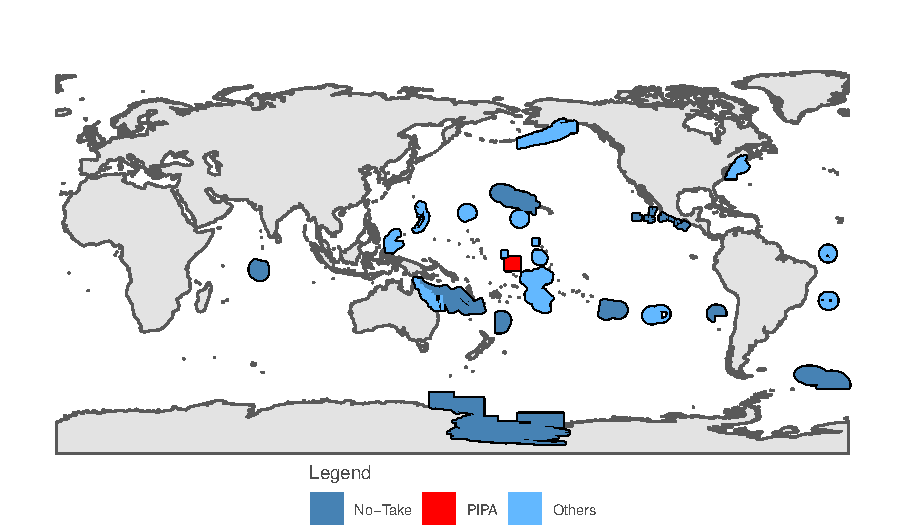
\includegraphics{img/LSMPAs_map.pdf}
\caption{\label{fig:LSMPAs_map}Large Scale Marine Protected Areas. The map shows all areas larger than 30,000 Km\textsuperscript{2}. The Phoenix Islands Protected Area is shown in red.}
\end{figure}

% PNA model output for costs
\begin{figure}[htbp]
\centering
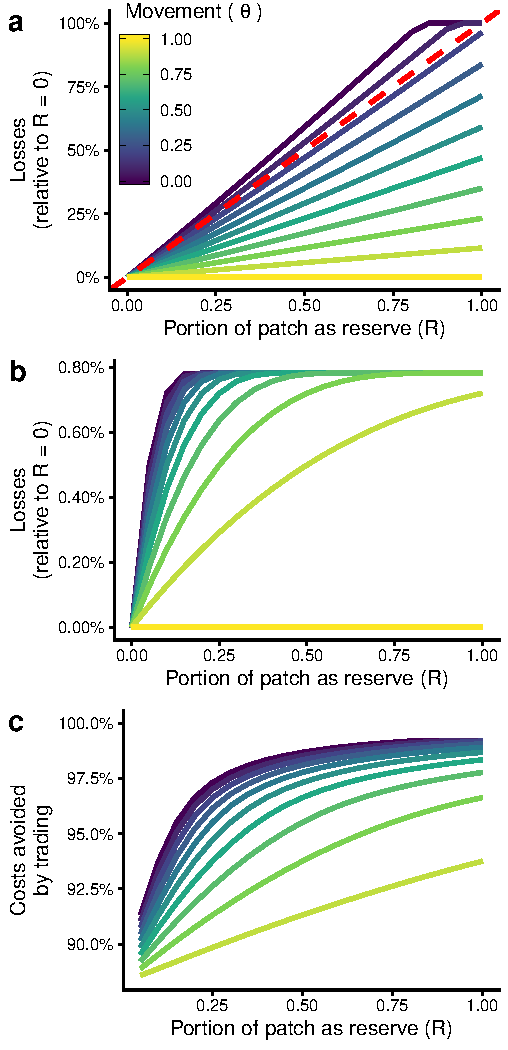
\includegraphics{img/PNA_model.pdf}
\caption{\label{fig:PNA_model}Cost of spatial closures in a vessel-day fishery (vertical axis) as a function of reserve size ($R$; horizontal axis) and movement ($\theta$; line color). Costs are shown for Patch 1 when there is no trading (A) and when trading is allowed (B). Costs avoided by tradig are shown in (C).}
\end{figure}

% Costs of different allocation rules
\begin{figure}[htbp]
\centering
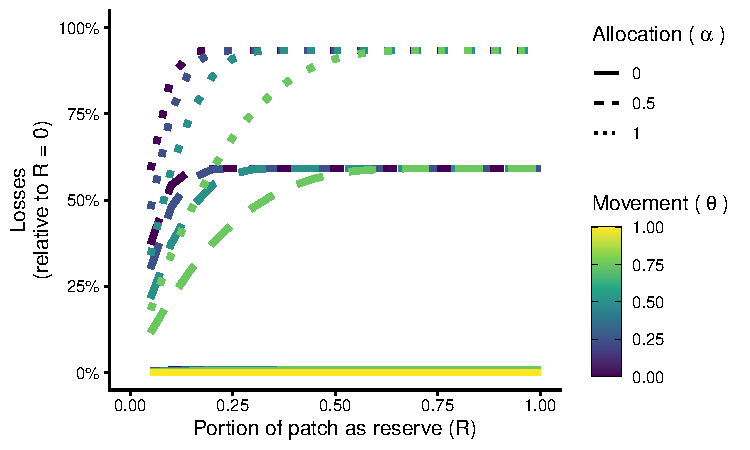
\includegraphics{img/allocation_cost_plot.pdf}
\caption{\label{fig:allocation_cost_plot}Cost (vertical axis) of different allocation rules (line colors) as a function of reserve  size ($R$; horizontal axis) and movement ($\theta$; line type). Costs are shown for Patch 1 only.}
\end{figure}

% Effort redistribution bars for Kiribati only
\begin{figure}[htbp]
\centering
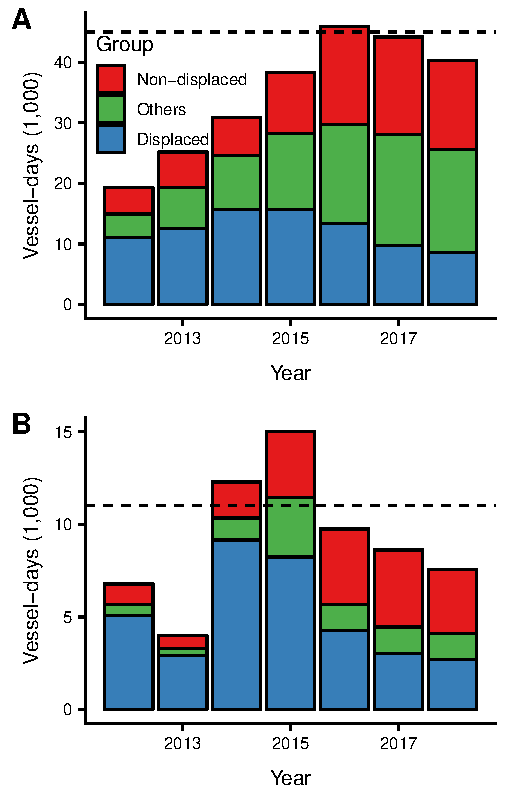
\includegraphics{img/all_PS_VDS_PNA_KIR_year.pdf}
\caption{\label{fig:all_PS_VDS_year}Observed vessel-days for all all PNA countries (A) and Kiribati (B) by displaced, non-displaced, and other vessels. Vessels displaced from PIPA fish less within the PNA, but non-displaced and other vessels fish more, resulting in a net increase. Vessels that used to fish within PIPA account for the largest effort reduction to Kiribati. The dashed horizontal lines represent the total allowable effort in the PNA (45,000 days) and Kiribati (11,000 days).}
\end{figure}

\begin{figure}[htbp]
\centering
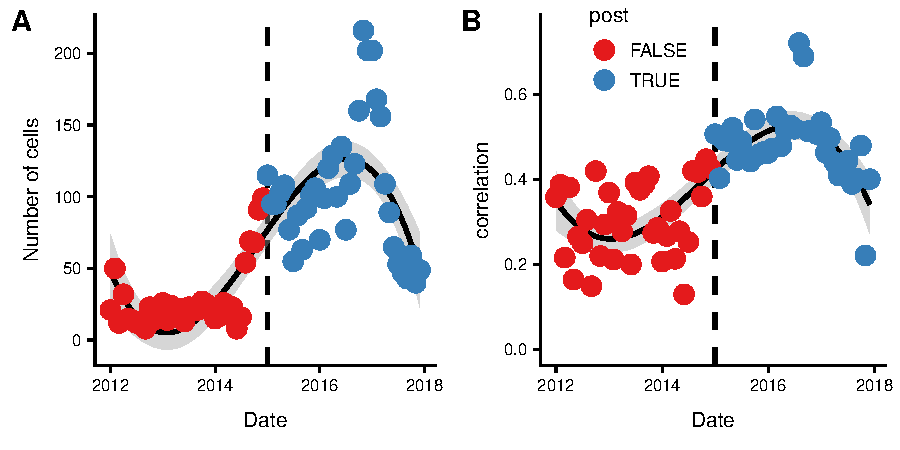
\includegraphics{img/sp_corr.pdf}
\caption{\label{fig:sp_corr}Number of cells that had displaced and non-displaced vessels (A) and spatial correlation in the presence-absence of each group per cell (B). The solid lines represent the 4\textsuperscript{th} degree polynomial fit reported in \ref{tab:sp_corr}. Note that the late 2016 and early 2017 showed negative or neutral NINO4 anomalies similar to those in the pre-PIPA period, but crowding effect does not decline to pre-implementation level and seems to stabilize.}
\end{figure}


\begin{figure}[htbp]
\centering
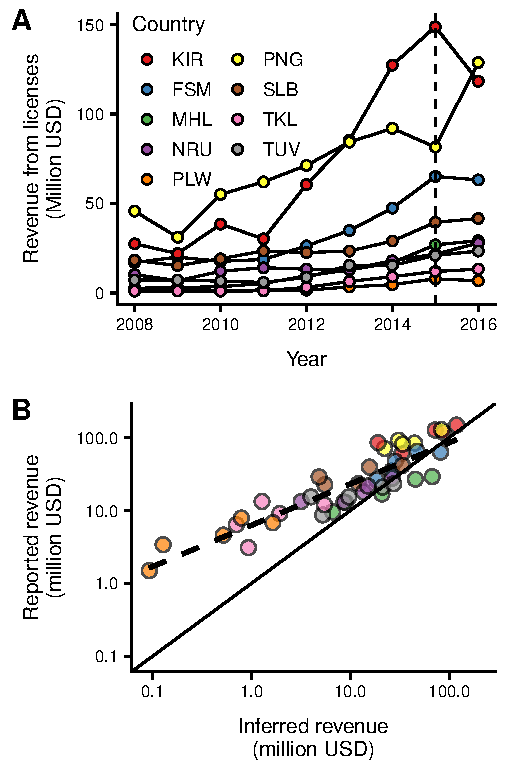
\includegraphics{img/revenues.pdf}
\caption{\label{fig:revenues}
License revenue for PNA countries. A) Annual revenue from fishing license fees by country and year (2008 - 2016) B) $log_{10}$-transformed FFA-reported revenues vs. the revenues inferred from vessel activity observations (2012 - 2016). The dashed line represents line of best fit, solid line represents 1:1 line. The same graph using absolute values is shown in \ref{fig:revenue_FFA_GFW_linear}.}
\end{figure}


%%%%%%%%%%%%%%%%%%%%%%%%%%%%%%%%%%%%%%%%%
%%%%%%%%%%%%%		 					 %%%%%%%%%%%%%
%%%%%%%%%%%%%		 BEGIN APPENDIX		 %%%%%%%%%%%%%
%%%%%%%%%%%%%		 					 %%%%%%%%%%%%%
%%%%%%%%%%%%%%%%%%%%%%%%%%%%%%%%%%%%%%%%%

\clearpage

\FloatBarrier

\newcommand{\beginsupplement}{\setcounter{table}{0}  \renewcommand{\thetable}{S\arabic{table}} \setcounter{figure}{0} \renewcommand{\thefigure}{S\arabic{figure}}}

\setcounter{table}{0}  \renewcommand{\thetable}{S\arabic{table}} \setcounter{figure}{0} \renewcommand{\thefigure}{S\arabic{figure}}

\section{Methods}

\subsection{Model for marine conservation with effort markets}

We model a ten-patch discrete-time meta-population system, where Patch 1 is considering a spatial closure. Patches 1 - 9 opperate under a vessel-day schemePatches, and Patch 10 represents the high seas and other areas not managed under a VDS. The stock of fish in each country is relatively stationary within a single fishing season, but redistributes across all patches annually. The price of fish is $p$, and catchability is given by $q$. These parameters are held constant across patches.

\subsubsection{Fishery dynamics}

In the absence of a reserve, the revenue for vessels in patch $i$ is given by $pqE_iX_i$, where $E_i$ and $X_i$ are effort (vessel-days) and stock size in patch $i$ at the beginning of a period. The cost of fishing in patch $i$ is given by $cE_i^\beta$, where $\beta = 1.3$ matches commonly-used cost functions.

Patch 1 considers a spatial closure by implementing a reserve as a fraction $R$ of the total patch ($R \in[0,1)$). Fish move within a patch based on $\theta$, where $\theta = 0$ implies no movement within the patch, and $\theta = 1$ implies that fish within the patch are well mixed during the fishing season. In this patch, revenues are given by $pqE_1X1(\theta + (1 - \theta)(1 - R))$. The parameterization of movement and reserve size imply that profit from fishing Patch 1 is given by:

$$
\Pi_1(E_1,X_1,R) = pqE_1X_1\Omega_i-cE_1^\beta
$$

With $\Omega_i = (\theta + (1 - \theta)(1 - R))$ being a parameterization that combines reserve size as a proportion of patch ($R =  (0, 1)$) and within-patch fish movement ($\theta$). Under this parameterization, $\Omega_{i \not 1} = 1$ since only Patch 1 implements a reserve.

Profits from fishing in each Patch are:

$$
\Pi_i(E_i,X_i) = pqE_iX_i\Omega_i-cE_i^\beta
$$

The above equations imply that the marginal profit from the last unit of effort in a patch are given by:

$$
\pi_1(E_1) = pqX_1\Omega_i - \beta cE_1^{\beta-1}
\label{eqn:marginal_profit}
$$

In practice, the effort levels in each Patch are allocated by management (so $E_{1},\ E_{2},...,E_{9}$ are given) and the
effort level on the high seas ($E_{10}$) is a result of open access dynamics. Therefore, we assume that effort continues to enter Patch 10 until the profit from the last unit of effort is exactly zero, indicating that $E_{10}$ is the value for which $\pi_{10}(E_{10})  = 0$. Setting Equation \ref{eqn:marginal_profit} for $i = 10$ equal to zero and removing $\Omega_{10} = 1$ for simplicity, we can solve for $E_{10}$:

$$
E_{10} = \left(\frac{pqX_{10}}{\beta c}\right)^{\frac{1}{(\beta - 1)}}
\label{eqn:effort_hs}
$$

Under vds-operated patches, however, profits from marginal effort must equate the cost of fishing in the patch. Therefore vessel-day price for patches under vds ($i = (1, 9)$) is  given by:

$$
\pi(E_i) = pqX_i\Omega_i - \beta c E_i ^{\beta - 1}
$$

We can solve for $E_i$ and obtain:

\begin{equation}
	\begin{split}
		\pi_i + \beta c E_i ^{\beta - 1} &= pqX_i\Omega_i \\
		\beta c E_i ^{\beta - 1} &= pqX_i\Omega_i - \pi_i \\
		E_i ^{\beta - 1} &= \frac{pqX_i\Omega_i - \pi_1}{\beta c} \\
		E_i &= \left(\frac{pqX_i\Omega_i - \pi_1}{\beta c }\right) ^ {\frac{1}{\beta - 1}}
	\end{split}
\label{eqn:demands}
\end{equation}

Therefore, total allowable effort in the fishery is given by:

$$
\bar{E} = \sum_{i = 1}^9\left(\frac{pqX_i\Omega_i - \pi}{\beta c }\right) ^ {\frac{1}{\beta - 1}}
\label{eqn:Ebar}
$$

\subsubsection{Stock dynamics}

Patch-level harvest is then determined by effort and stock size:

$$
H_i = qE_iX_i\Omega_i
\label{eqn:harvest}
$$

Therefore, escapement in patch $i$ is the difference between initial stock size and harvests given by $e_{it} = X{it} - H_{it}$ and total escapement is $e_t=\sum_{i=1}^{10}e_{it}$. The entire stock then grows logistically according to:

$$
X_{t+1} = e_t + e^{r \times \frac{e}{K}}
\label{eqn:grow}
$$

Where $r$ and $K$ are species-specific intrinsic growth rate and carrying capacity.

After the stock grows, a constant and patch-specific fraction $f_i$ of the total stock redistributes to patch $i$, so:

$$
X_{it+1} = f_iX_{t+1}
\label{eqn:disperse}
$$

\subsubsection{Vessel-day revenues}

The vessel-day price that a country charges is given by $\pi_i$ from Eqn \ref{eqn:marginal_profit}. Therefore, patch-level license revenues are given by:

$$
\omega = \pi_iE_i
\label{eqn:license_revenue}
$$

Equation \ref{eqn:harvest} shows that low values of $\theta$ and $R > 0$ would increase escapement, which would lead to an increase in stock size (Equation \ref{eqn:grow}) and a benefit to all the other patches. But this would also cause the stock in the high seas ($X_{10}$) to increase, leading to an increased effort being allocated to the high seas (Equation \ref{eqn:effort_hs}) and a loss of these potential rents. Thus, the spillover benefits of increasing $R$ are never completely captured.

\subsubsection{Simulations and parametrization}

We inform our model to losely match the fishery dynamics observed for the VDS operated by the PNA. The table below contains the values used to parameterize the model.


\begin{tabular}{l|r|l}
\hline
Parameter & Value & Source\\
\hline
MSY & 1.875600e+06 & 50th percentile from MSY in table 8 of Stock Assessment\\
\hline
$B_{msy}$ & 1.628000e+06 & 50th percentile from MSY in table 8 of Stock Assessment\\
\hline
K & 6.876526e+06 & 50th percentile from MSY in table 8 of Stock Assessment\\
\hline
$B_c/B_{msy}$ & 5.100000e-01 & 50th percentile from MSY in table 8 of Stock Assessment\\
\hline
$C_{now}$ & 1.679444e+06 & Catches from Stock Assessment\\
\hline
$B_{now}$ & 3.507028e+06 & Current Biomass (2012 - 2015 average)\\
\hline
$r$ & 5.700000e-01 & From fishbase: Prior r = 0.57, 95 CL = 0.41 - 0.78\\
\hline
$\beta$ & 1.300000e+00 & Standard\\
\hline
p & 1.100000e+03 & Mean between Thailand and Japan values (Value of WCPFC-CA tuna fisheries 2017 report)\\
\hline
q & 3.420000e-05 & Estimated so that efforts match catches given biomass and vessel-day prices\\
\hline
c & 1.800000e+02 & -\\
\hline
f & 1.000000e-01 & Biomass is equally distributed between patches ($f_i = 0.1$)\\
\hline
\end{tabular}

We use the model above run three different simulations. We test the model across a range reserve sizes and movement parameters. We use to main scenarios. The first scenario does not allow trading. In this case, total allowable effort ($\bar{E}$) and biomass $B_{now}$ are known and equally distributed among patches 1-9. For patch 10, we solve for Eq \ref{eqn:effort_hs} until biomass converges to match $B_{now}$. We then proceed to ``close'' a portion of Patch 1, and calculate the vessel-day price in Patch 1 given that only $X_i\Omega_i$ biomass is available for harvest. We compare vessel-day revenues of each scenario to a case with no reserve ($R = 0$). This produces a measure of the cost of implementing a spatial closure of size $R$ in patch 1.

The second scenario allows trading. We start again by solving for the high seas to obtain total effort. Since a closure is not in effect, this equiulibrium is the same as the first step above. We then implement a spatial closure in patch 1. This essentially lowers the price fishers would be willing to pay to fish in a patch with biomass $X_i\Omega_i$, lowering demand for vessel-days in pach 1. Patches 2 - 9 have a higher demand for vessel days, and therefore a portion of vessel-days from patch 1 are sold to patches 2 - 9. This increases effort in these patches, which reduces escapement and therefore biomass. This reduction in biomass in turn would modify the demand curves (Eq \ref{eqn:demands}). We therefore iterate this process until biomass stabilizes, therefore finding the system's equilibrium. Like before, we calculate vessel-day revenues to each patch and compare them to a case with no reserve in patch 1.

\subsection{Allocation rules}

In the second scenario above, effort from a patch with conservation is traded to other patches. This means that its allocation will decrease as purse seine effort in its EEZ is reduced. After solving for the new equilibrium for each combination of $R$ and $\theta$, we project the fishery 50 years in time. At the end of every time, vessel-days are allocated to each patch based on the following rule:

$$
E_i^* = \alpha \left(\frac{\sum_{\tau = 0}^{\hat{\tau}}E_{i,t-\tau}}{\bar{E}\hat{\tau}} \right) +
(1 - \alpha) \left(\frac{\sum_{\tau = 0}^{\hat{\tau}}X_{i,t-\tau}}{\bar{X}\hat{\tau}} \right)
$$

Where  $\alpha$ is a weight on historical effort ($E_i$) and $1-\alpha$ is the weight in historical biomass ($B_i$). We use $\hat{\tau}= 7$ to obtain a moving mean of 7 years for these measures. The difference between allocated days ($E_i^*$) and used days (determined by Eq: \ref{eqn:demands}) for patch 1 are the sales. We then calculate vessel-day revenues to each country over the 50-year time horizon and compare them to a case where there is no reserve and allocations are based solely on biomass ($\alpha = 0$).

\subsection{Data}

Automatic Identification Systems (AIS) are on-board devices that provide at-sea safety and prevent ship collisions by broadcasting vessel position, course, and activity to surrounding vessels. These broadcast messages can be received by satellites and land-based antennas. GFW then uses machine learning algorithms (convolutional neural networks) on the broadcast messages to infer type and location of fishing events \cite{kroodsma_2018}.

The amount of data gathered by GFW is dependent on the number of antennas and satellites that can receive signals. The total satellite count increased from 3 to 6 on June 1\textsuperscript{st} 2014 , and then from 6 to 10 on January 1\textsuperscript{st} 2016. This causes an increase in the number of \emph{received} AIS messages (\emph{i.e.} points), and therefore an apparent increase in the number of vessels and vessel activity. The addition of new satellites affects all vessels in the same way.

Our displaced group contains all purse seiners (n = 64) that fished within PIPA at least once before the announcement, and that continued to fish elsewhere after the January 2015 implementation. Vessels in the non-displaced group meet the following two conditions: i) never fished within PIPA waters from 2012-2015, and ii) vessels have fished in surrounding areas (\emph{i.e.} PNA-countries' EEZ) before and after PIPA closure (n = 28). Together, these vessels represent more than 20 million geo-referenced positions for which we know activity (fishing or not fishing). We perform three sample restrictions as a robustness check. The first restriction excludes all Chinese vessels, the second excludes all PNA vessels, and the third excludes US and Taiwanese vessels. 

\clearpage

\subsection{Analysis}

\subsubsection{Crowding effect}

$$
y_t = \alpha + \beta_1 M_t + \beta_2 M_t^2 + \beta_3 M_t^3 + \beta_4 M_t ^4 + \sigma_s + \mu N_t + \epsilon_t
\label{eqn:sp_corr}
$$

We test for a crowding effect using the specification in Equation [\ref{eqn:sp_corr}]. We have two different outcome variables:
1) the number of cells that had fishing activity from displaced and non-displaced vessels per month and 2) the correlation of presence/absence of fishing events between both groups over one month.We allow for the possibility of three inflection points: 1) initial crowding due to MPA implementation, 2) When the crowding has reached its peak and starts to decrease, and 3) when this decrease potentially levels off. For this reason, we fit a 4th degree polynomial to our monthly indices. We do so by centering our time series of crowding indices on the day of implementation. Our explanatory variable is therefore the number of months ($M$) before or after the implementation. For example, since PIPA was implemented in January 1st of 2015, December of 2014 has a value of -1 and Feb of 2015 would receive a value of 1. Note that we restrict the sample to our displaced and non-displaced vessels (vessels that show up in the dataset before PIPA implementation) to try to minimize bias from more and more vessels using AIS over time. We also include controls ($\sigma_s$) that captures the effect of additional satellites receiving AIS signals, which occurred on April 1st, 2014 and December 31st, 2015. The $\mu$ coefficient captures the effect of the NINO4 anomaly.

\subsubsection{Behavioral changes}

We attempt to identify the response of vessels to the PIPA closure. We use daily fishing and non-fishing hours, daily proportion of fishing vs. non-fishing hours, daily distance traveled (km), distance from shore (km) and distance from home port (km) for fishing events, and proportion of total fishing hours allocated to Kiribati waters and PNA waters as our main outcomes of interest. We compare these outcomes before and after the implementation of PIPA using a Difference-in-Differences approach. 

Our main specification is the following:

$$
log(y_{i,t}) = \alpha + \beta_1 P_t + \beta_2 D_i + \beta_3 P_t \times D_i + \phi_t + \gamma_i + \epsilon_{i,t}
\label{eqn:did}
$$

\noindent where $log(y_{i,t})$ is the hyperbolic-sine transformation\footnote{$ln\left(y + \sqrt{1 + y^2}\right)\rightarrow ln(2y)$ the transformation was not applied to the proportion of fishing to non-fishing hours.} of the outcome of interest for vessel $i$ on period $t$. A dummy variable $P_t$ takes the value of 0 for all dates prior to PIPA implementation and a value of 1 for all dates following PIPA implementation. $D_i$ is a dummy variable indicating whether a vessel belongs to the displaced ($D_i = 1$) or non-displaced ($D_i = 0$) group. $\alpha$ is the standard intercept term, $\beta_1$ captures the temporal trend, $\beta_2$ captures the initial difference between displaced and non-displaced groups, and $\beta_3$ is our parameter of interest: the difference-in-differences estimate capturing the treatment effect. Finally, $\phi_t$ and $\gamma_i$ represent month and flag dummies that account for seasonality or country-level management interventions. 

All regression coefficients were estimated via ordinary least squares, and heteroskedasticity-robust standard errors were calculated. All analyses were performed in R version 3.5.1 \cite{rcore_2018}. Raw data and code used in this work are available on \href{https://github.com/jcvdav/MPA_displacement}{github}.

\subsubsection{Revenues and catches}

We obtained information on revenues from the Pacific Islands Forum Fisheries Agency \emph{Tuna Development Indicators 2016} report.  Specifically, we use data compiled by the Pacific Islands Forum Fisheries Agency (FFA\footnote{https://www.ffa.int/node/2050}) where annual revenues from license fees (for VDS and other access programs) are reported for each country (2008 - 2016; Fig. \ref{fig:revenues}A). For countries in the PNA, these revenues show a combination of vessel-day license fees as well as joint-venture operations.

Total purse seine catch for each country's EEZ for the 1997 - 2016 period were also obtained from the FFA (Fig. \ref{fig:catches}). Catches in Kiribati waters decreased from 24,051 to 12,894 tonnes between 2015 and 2016 (46.3\% decrease). Similar decreases were observed for The Federated States of Micronesia (60.9\%), Papua New Guinea (43.4\%) and the Solomon Islands (58.5\%). In contrast, Tokelau (due south of PIPA) showed a 22.3\% increase in purse seine catch over the same period.

\clearpage

\section{Supplementary tables and figures}

\begin{figure}[H]
\centering
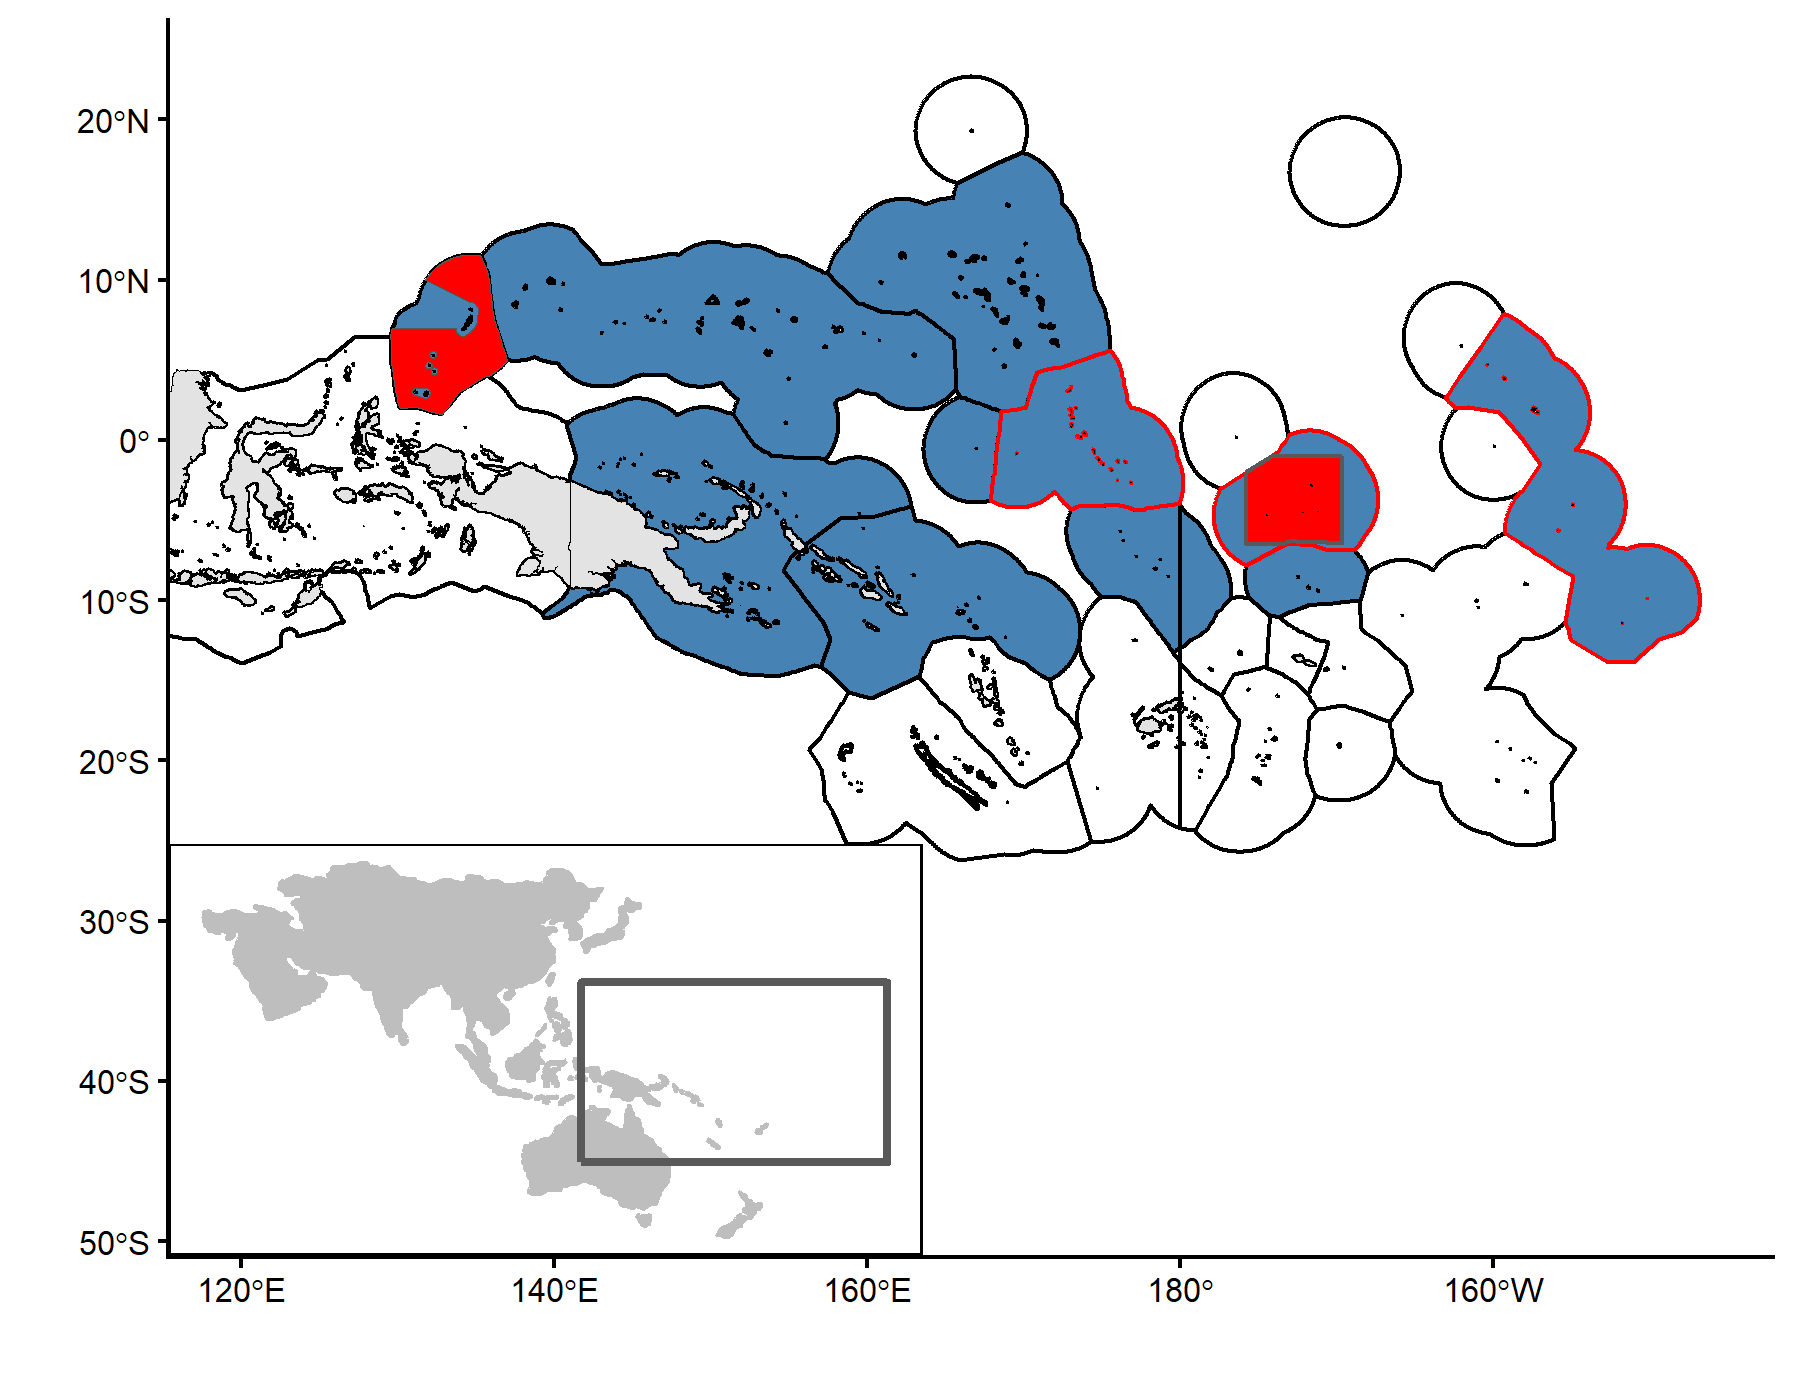
\includegraphics{img/PNA_map.png}
\caption{\label{fig:PNA_map}Map of the Exclusive Economic Zones (EEZs) of the region of interest. Countries that belong to the PNA are shown in blue, while empty polygons indicate all others. A red line indicates the Kiribati EEZ, and a solid red polygon shows PIPA. A solid purple polygon shows PNMS. Land masses are shown in gray. Labels indicate ISO3 country codes (PLW: Palau, PNG: Papua New Guinea, FSM: Federal States of Micronesia, SLB: Solomon Islands, NRU: Nauru, MHL: Marshal Islands, KIR: Kiribati, TUV: Tuvalu, TKL: Tokelau).}
\end{figure}

\begin{figure}
\centering
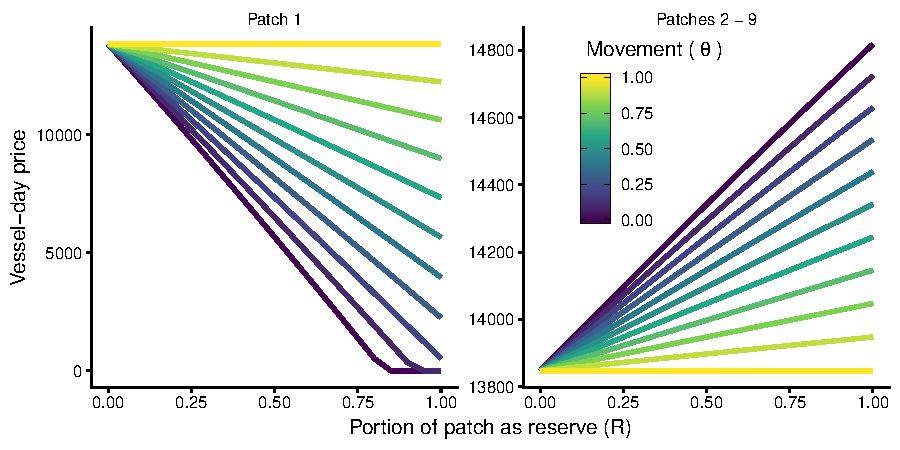
\includegraphics{img/vessel_day_price_no_trading_plot.pdf}
\caption{\label{fig:vessel_day_price_no_trading_plot}Vessel-day prices (vertical axis) for a combination of reserve sizes ($R$ in the horizontal-axis) and different within-patch movement ($theta$) for the patch with spatial closure and other patches (left - right, respectively) when there is no trading.}
\end{figure}

\begin{figure}
\centering
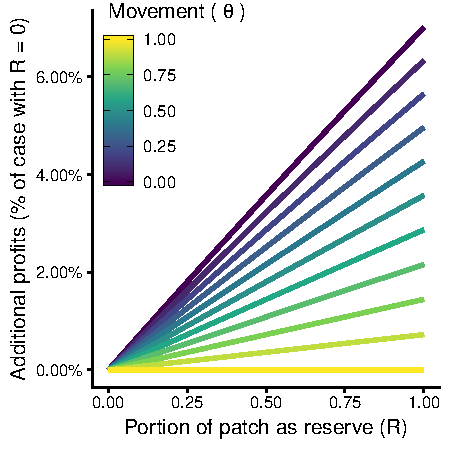
\includegraphics{img/profits_PNA_notKIR_no_trading_plot.pdf}
\caption{\label{fig:profits_PNA_notKIR_no_trading_plot}Relative change in revenue for patches 2 - 9 (vertical axis) for a combination of reserve sizes ($R$ in the horizontal-axis) and different within-patch movement ($theta$) when there is no trading.}
\end{figure}

\begin{figure}
\centering
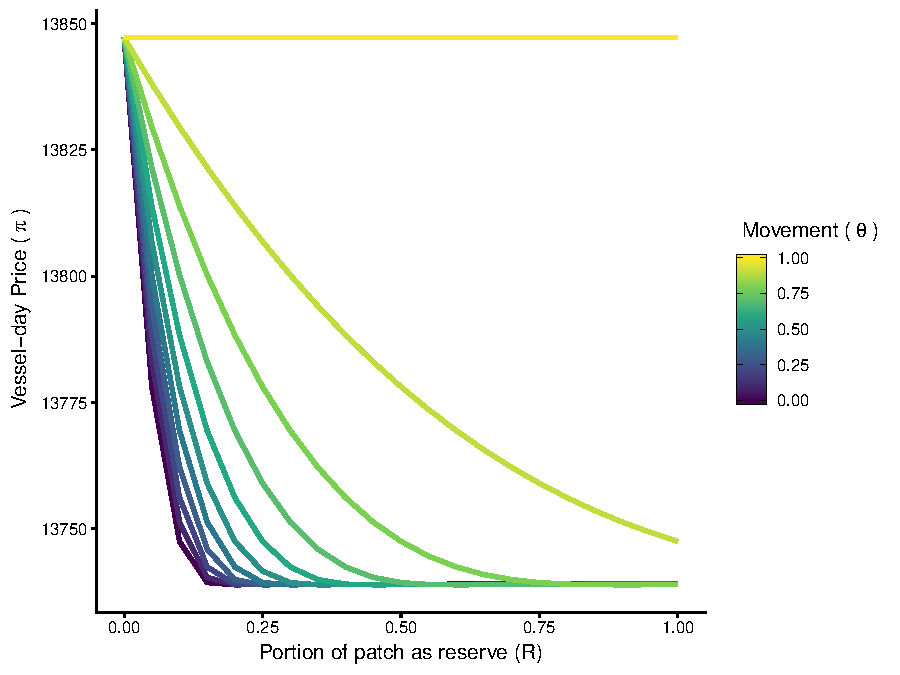
\includegraphics{img/vessel_day_price_with_trading_plot.pdf}
\caption{\label{fig:vessel_day_price_with_trading_plot}Vessel-day prices (vertical axis) for a combination of reserve sizes ($R$ in the horizontal-axis) and different within-patch movement ($theta$) for the patch with spatial closure and other patches (left - right, respectively) when there is no trading.}
\end{figure}

\begin{figure}
\centering
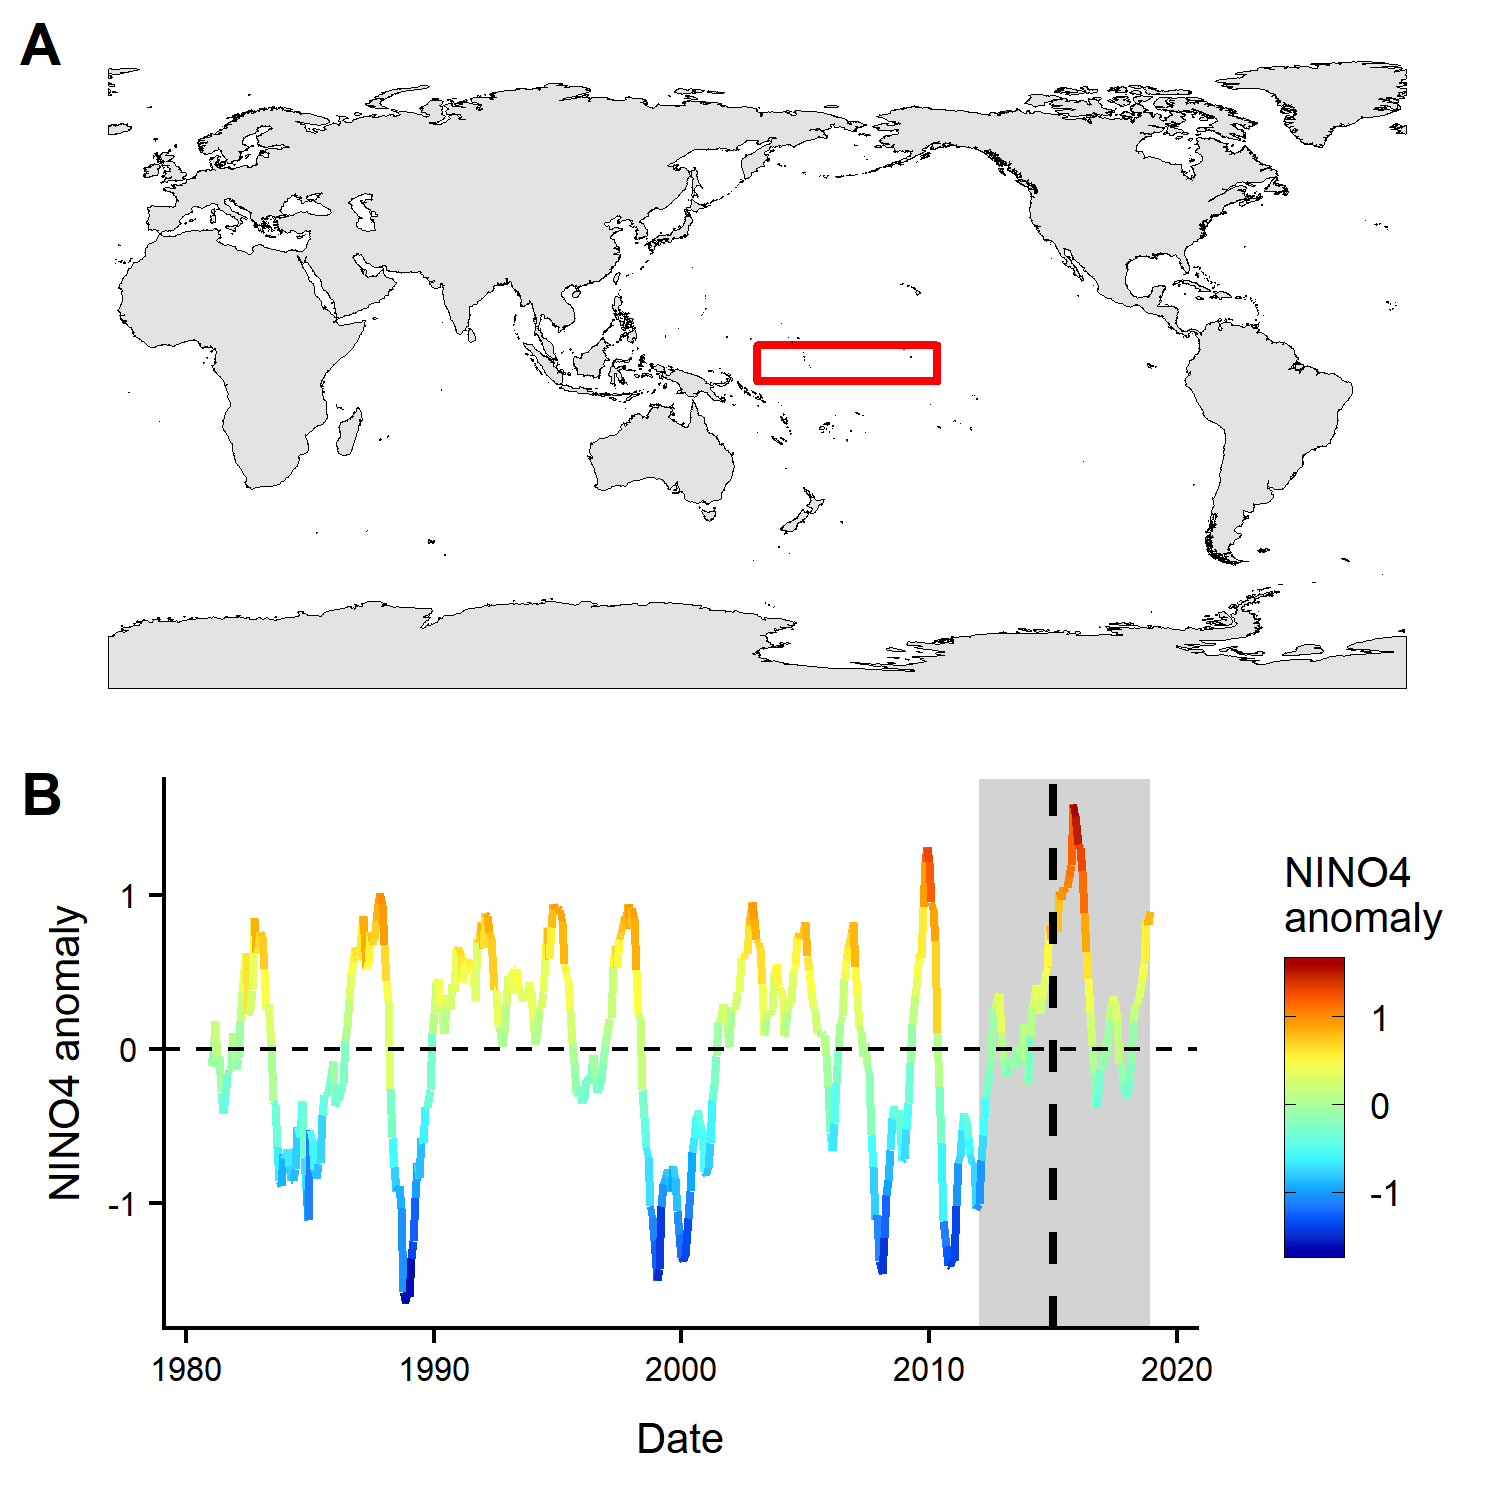
\includegraphics{img/nino_plot.png}
\caption{\label{fig:nino_plot}NINO4 anomaly index. A) Map of the NINO4 region (5S-5N and 160E-150W). B) Timeseries of NINO4 anomaly from January, 1980 to December, 2018.}
\end{figure}

\clearpage

\begin{figure}
\centering
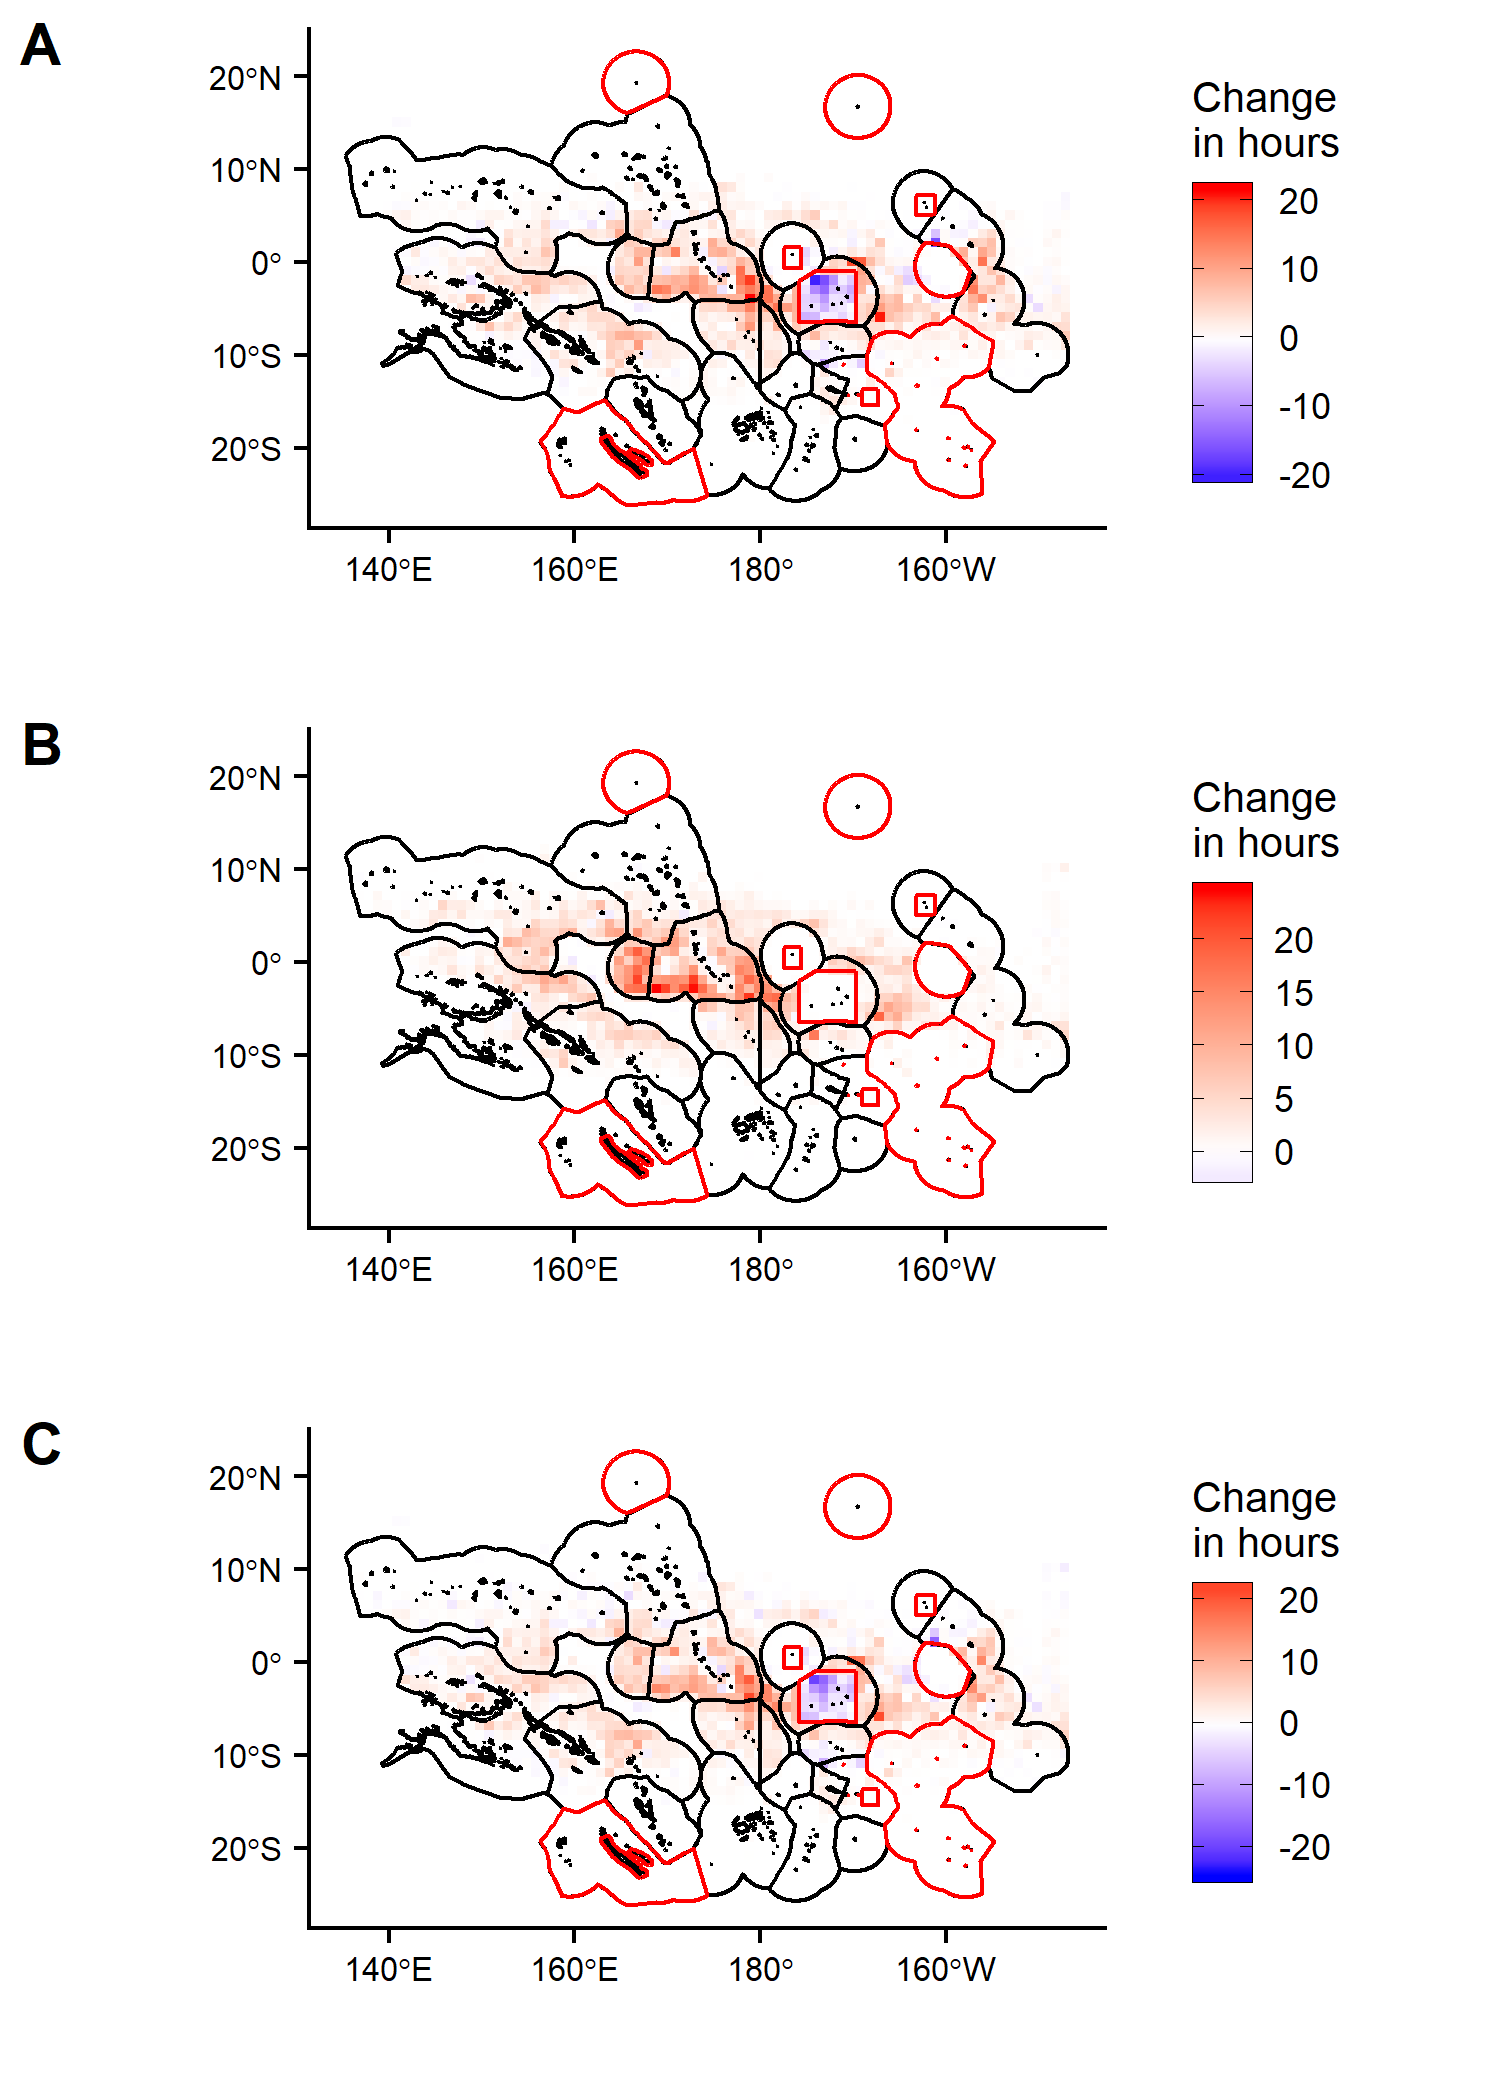
\includegraphics{img/fishing_raster_diff.png}
\caption{\label{fig:fishing_raster_diff}Change in spatial footprint of analyzed vessels. Black lines show Exclusive Economic Zone (EEZ), red lines show existing Marine Protected Areas. Panels A and B show the change through time (after - before) for displaced (A) and non-displaced vessels (B). Panel C shows the difference between A and B (displaced - non-displaced), highlighting areas where displaced vessels redistributed to, relative to non-displaced vessels. Note that displaced vessels allocate more hours to the Gilbert Islands and Line islands EEZs, but also Tuvalu and the high seas surrounding PIPA and Kiribati's EEZ.}
\end{figure}

\begin{landscape}

\begin{table}[!htbp] \centering 
  \caption{\label{tab:sp_corr}Coefficient estimates for a third-polinomial fit to the measures of crowding. The first column shows coefficients for the number of cells with treated and control vessels during the same month. The second column shows coefficients for the spatial correlation for presence / absence of treated and control vessels. The explanatory variable is the number of months before implementation of PIPA. Numbers in parentheses are heteroskedastic-robust standard errors.} 
  \label{} 
\footnotesize 
\begin{tabular}{@{\extracolsep{1pt}}lcccccccc} 
\\[-1.8ex]\hline 
\hline \\[-1.8ex] 
\\[-1.8ex] & (1) & (2) & (3) & (4) & (5) & (6) & (7) & (8)\\ 
\hline \\[-1.8ex] 
 Constant & 78.040$^{***}$ & 84.639$^{***}$ & 60.962$^{***}$ & 66.725$^{***}$ & 0.412$^{***}$ & 0.417$^{***}$ & 0.370$^{***}$ & 0.377$^{***}$ \\ 
  & (5.438) & (8.990) & (15.598) & (15.988) & (0.014) & (0.032) & (0.062) & (0.066) \\ 
  & & & & & & & & \\ 
 M & 3.943$^{***}$ & 4.065$^{***}$ & 3.066$^{***}$ & 3.139$^{***}$ & 0.010$^{***}$ & 0.010$^{***}$ & 0.009$^{**}$ & 0.009$^{**}$ \\ 
  & (0.302) & (0.348) & (0.966) & (1.040) & (0.001) & (0.001) & (0.003) & (0.004) \\ 
  & & & & & & & & \\ 
 M $^2$ & $-$0.005 & $-$0.021 & 0.008 & $-$0.008 & $-$0.0001$^{***}$ & $-$0.0001 & $-$0.0001 & $-$0.0001 \\ 
  & (0.019) & (0.026) & (0.027) & (0.030) & (0.00004) & (0.0001) & (0.0001) & (0.0001) \\ 
  & & & & & & & & \\ 
 M $^3$ & $-$0.002$^{***}$ & $-$0.002$^{***}$ & $-$0.002$^{***}$ & $-$0.002$^{***}$ & $-$0.00001$^{***}$ & $-$0.00001$^{***}$ & $-$0.00001$^{***}$ & $-$0.00001$^{***}$ \\ 
  & (0.0003) & (0.0003) & (0.001) & (0.001) & (0.00000) & (0.00000) & (0.00000) & (0.00000) \\ 
  & & & & & & & & \\ 
 M $^4$ & 0.00001 & 0.00002 & 0.00000 & 0.00001 & 0.00000$^{***}$ & 0.00000$^{**}$ & 0.00000 & 0.00000 \\ 
  & (0.00001) & (0.00002) & (0.00002) & (0.00002) & (0.00000) & (0.00000) & (0.00000) & (0.00000) \\ 
  & & & & & & & & \\ 
 NINO4 &  & $-$8.095 &  & $-$10.395 &  & $-$0.006 &  & $-$0.014 \\ 
  &  & (8.287) &  & (9.481) &  & (0.029) &  & (0.031) \\ 
  & & & & & & & & \\ 
 $\sigma_1$ &  &  & 21.318 & 25.102 &  &  & 0.057 & 0.062 \\ 
  &  &  & (19.493) & (22.486) &  &  & (0.076) & (0.080) \\ 
  & & & & & & & & \\ 
 $\sigma_2$ &  &  & 5.299 & 3.194 &  &  & $-$0.015 & $-$0.018 \\ 
  &  &  & (18.874) & (18.670) &  &  & (0.035) & (0.035) \\ 
  & & & & & & & & \\ 
\hline \\[-1.8ex] 
NINO4 & No & Yes & No & Yes & No & Yes & No & Yes \\ 
Satellites & No & No & Yes & Yes &  &  &  &  \\ 
Observations & 84 & 84 & 84 & 84 & 84 & 84 & 84 & 84 \\ 
R$^{2}$ & 0.791 & 0.793 & 0.795 & 0.798 & 0.703 & 0.704 & 0.709 & 0.710 \\ 
\hline 
\hline \\[-1.8ex] 
\textit{Note:}  & \multicolumn{8}{r}{$^{*}$p$<$0.1; $^{**}$p$<$0.05; $^{***}$p$<$0.01} \\ 
\end{tabular} 
\end{table} 

\end{landscape}

\begin{landscape}

\begin{table}[H] \centering 
  \caption{\label{tab:KIR_sp_corr}Coefficient estimates for a fourth-degree polynomial fit to the measures of crowding for Kiribati EEZ only. The first five columns represent different specifications for number of cells with presence of both fleets. Columns 6 - 10 show coefficients for the spatial correlation for presence / absence of displaced and non-displaced vessels. The explanatory variable is the number of months before or after implementation of PIPA. Numbers in parentheses are heteroskedastic-robust standard errors. The last column of each group presents fits with only NINO4 anomaly index as an explanatory variable.} 
  \label{} 
\footnotesize 
\begin{tabular}{@{\extracolsep{0.1pt}}lcccccccccc} 
\\[-1.8ex]\hline 
\hline \\[-1.8ex] 
\\[-1.8ex] & \multicolumn{5}{c}{Number of cells} & \multicolumn{5}{c}{Pearson's correlation coefficient} \\ 
\\[-1.8ex] & (1) & (2) & (3) & (4) & (5) & (6) & (7) & (8) & (9) & (10)\\ 
\hline \\[-1.8ex] 
 Constant & 30.24$^{***}$ & 32.77$^{***}$ & 23.30$^{***}$ & 26.14$^{***}$ & 16.23$^{***}$ & 0.43$^{***}$ & 0.43$^{***}$ & 0.33$^{***}$ & 0.34$^{***}$ & 0.38$^{***}$ \\ 
  & (2.43) & (4.16) & (4.59) & (5.49) & (2.37) & (0.03) & (0.05) & (0.07) & (0.08) & (0.03) \\ 
  & & & & & & & & & & \\ 
 M & 1.29$^{***}$ & 1.34$^{***}$ & 1.00$^{***}$ & 1.06$^{***}$ &  & 0.01$^{***}$ & 0.01$^{***}$ & 0.01$^{*}$ & 0.01 &  \\ 
  & (0.14) & (0.17) & (0.27) & (0.30) &  & (0.002) & (0.002) & (0.01) & (0.01) &  \\ 
  & & & & & & & & & & \\ 
 M $^2$ & $-$0.03$^{***}$ & $-$0.04$^{***}$ & $-$0.02$^{**}$ & $-$0.03$^{***}$ &  & 0.0000 & 0.0000 & 0.0001 & 0.0001 &  \\ 
  & (0.01) & (0.01) & (0.01) & (0.01) &  & (0.0002) & (0.0002) & (0.0002) & (0.0002) &  \\ 
  & & & & & & & & & & \\ 
 M $^3$ & $-$0.001$^{***}$ & $-$0.001$^{***}$ & $-$0.001$^{***}$ & $-$0.001$^{***}$ &  & $-$0.0000$^{***}$ & $-$0.0000$^{***}$ & $-$0.0000$^{**}$ & $-$0.0000$^{**}$ &  \\ 
  & (0.0001) & (0.0001) & (0.0002) & (0.0002) &  & (0.0000) & (0.0000) & (0.0000) & (0.0000) &  \\ 
  & & & & & & & & & & \\ 
 M $^4$ & 0.0000$^{***}$ & 0.0000$^{***}$ & 0.0000$^{**}$ & 0.0000$^{***}$ &  & $-$0.0000 & $-$0.0000 & $-$0.0000 & $-$0.0000 &  \\ 
  & (0.0000) & (0.0000) & (0.0000) & (0.0000) &  & (0.0000) & (0.0000) & (0.0000) & (0.0000) &  \\ 
  & & & & & & & & & & \\ 
 NINO4 &  & $-$3.10 &  & $-$4.19 & 9.93$^{***}$ &  & $-$0.001 &  & $-$0.02 & 0.11$^{***}$ \\ 
  &  & (3.97) &  & (4.16) & (3.33) &  & (0.05) &  & (0.06) & (0.03) \\ 
  & & & & & & & & & & \\ 
 $\sigma_1$ &  &  & 9.40 & 10.33 &  &  &  & 0.12 & 0.13 &  \\ 
  &  &  & (5.92) & (6.35) &  &  &  & (0.09) & (0.09) &  \\ 
  & & & & & & & & & & \\ 
 $\sigma_2$ &  &  & $-$2.46 & $-$3.84 &  &  &  & 0.02 & 0.01 &  \\ 
  &  &  & (5.70) & (5.77) &  &  &  & (0.10) & (0.11) &  \\ 
  & & & & & & & & & & \\ 
\hline \\[-1.8ex] 
NINO4 & No & Yes & No & Yes & Yes & No & Yes & No & Yes & Yes \\ 
Satellites & No & No & Yes & Yes & No &  &  &  &  &  \\ 
AIC & 654.294 & 655.536 & 655.482 & 656.125 & 724.58 & -65.872 & -63.873 & -63.481 & -61.572 & -35.895 \\ 
Observations & 84 & 84 & 84 & 84 & 84 & 75 & 75 & 75 & 75 & 75 \\ 
R$^{2}$ & 0.63 & 0.63 & 0.64 & 0.65 & 0.08 & 0.44 & 0.44 & 0.45 & 0.45 & 0.09 \\ 
\hline 
\hline \\[-1.8ex] 
\textit{Note:}  & \multicolumn{10}{r}{$^{*}$p$<$0.1; $^{**}$p$<$0.05; $^{***}$p$<$0.01} \\ 
\end{tabular} 
\end{table} 

\end{landscape}

\begin{figure}
\centering
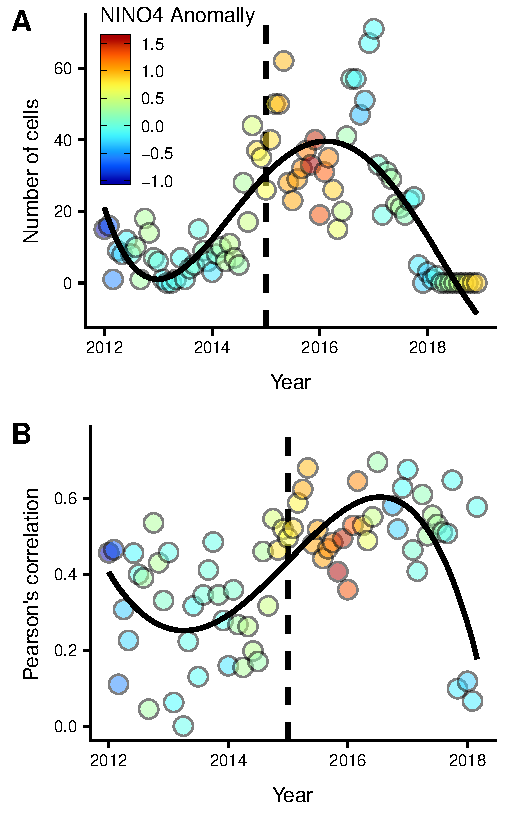
\includegraphics{img/KIR_sp_corr.pdf}
\caption{\label{fig:KIR_sp_corr}Number of cells that had displaced and non-displaced vessels (A) and spatial correlation in the presence-absence of each group per cell (B) for Kiribati's EEZ only. The solid lines represent the 4\textsuperscript{th} degree polynomial fit reported in \ref{tab:sp_corr}. Note that the late 2016 and early 2017 showed negative or neutral NINO4 anomalies, similar to those in the pre-PIPA period.}
\end{figure}

\begin{landscape}

\begin{table}[!htbp] \centering 
  \caption{\label{tab:main_DID}Difference-in-differences estimates for our 10 variables of interest: 1) Daily fishing hours, 2) Daily non-fishing at-sea hours, 3) Daily proportion of fishing hours to total at-sea hours, 4) Daily distance traveled, 5) Daily mean distance from port for fishing events, 6) Daily mean distance from shore for fishing events, 7) Monthly fishing hours spent in Kiribati waters, 8) Monthly fishing hours spent in PNA waters. Numbers in parentheses are heteroskedastic-robust standard errors.} 
  \label{} 
\footnotesize 
\begin{tabular}{@{\extracolsep{1pt}}lcccccccc} 
\\[-1.8ex]\hline 
\hline \\[-1.8ex] 
\\[-1.8ex] & (1) & (2) & (3) & (4) & (5) & (6) & (7) & (8)\\ 
\hline \\[-1.8ex] 
 Constant & 0.497$^{***}$ & 3.607$^{***}$ & 0.075$^{***}$ & 5.203$^{***}$ & 12.997$^{***}$ & 12.461$^{***}$ & 3.678$^{***}$ & 4.445$^{***}$ \\ 
  & (0.022) & (0.012) & (0.004) & (0.029) & (0.021) & (0.019) & (0.192) & (0.151) \\ 
  & & & & & & & & \\ 
 Post & 0.839$^{***}$ & $-$0.228$^{***}$ & 0.137$^{***}$ & 0.304$^{***}$ & 0.326$^{***}$ & 0.296$^{***}$ & 1.059$^{***}$ & 1.180$^{***}$ \\ 
  & (0.016) & (0.008) & (0.003) & (0.019) & (0.014) & (0.014) & (0.140) & (0.109) \\ 
  & & & & & & & & \\ 
 Treated & 0.136$^{***}$ & 0.014$^{**}$ & 0.015$^{***}$ & 0.400$^{***}$ & 0.223$^{***}$ & 0.116$^{***}$ & 0.534$^{***}$ & 0.149 \\ 
  & (0.013) & (0.007) & (0.002) & (0.020) & (0.016) & (0.016) & (0.148) & (0.118) \\ 
  & & & & & & & & \\ 
 Post $\times$ Treated & $-$0.244$^{***}$ & 0.013 & $-$0.034$^{***}$ & $-$0.483$^{***}$ & $-$0.281$^{***}$ & $-$0.155$^{***}$ & $-$0.565$^{***}$ & $-$0.399$^{***}$ \\ 
  & (0.019) & (0.009) & (0.003) & (0.022) & (0.017) & (0.017) & (0.161) & (0.127) \\ 
  & & & & & & & & \\ 
\hline \\[-1.8ex] 
Month FE & Yes & Yes & Yes & Yes & Yes & Yes & Yes & Yes \\ 
Flag FE & Yes & Yes & Yes & Yes & Yes & Yes & Yes & Yes \\ 
Observations & 83,052 & 83,052 & 83,051 & 64,387 & 32,055 & 32,055 & 1,814 & 2,588 \\ 
R$^{2}$ & 0.102 & 0.072 & 0.107 & 0.028 & 0.062 & 0.080 & 0.113 & 0.198 \\ 
\hline 
\hline \\[-1.8ex] 
\textit{Note:}  & \multicolumn{8}{r}{$^{*}$p$<$0.1; $^{**}$p$<$0.05; $^{***}$p$<$0.01} \\ 
\end{tabular} 
\end{table} 

\end{landscape}

\begin{figure}
\centering
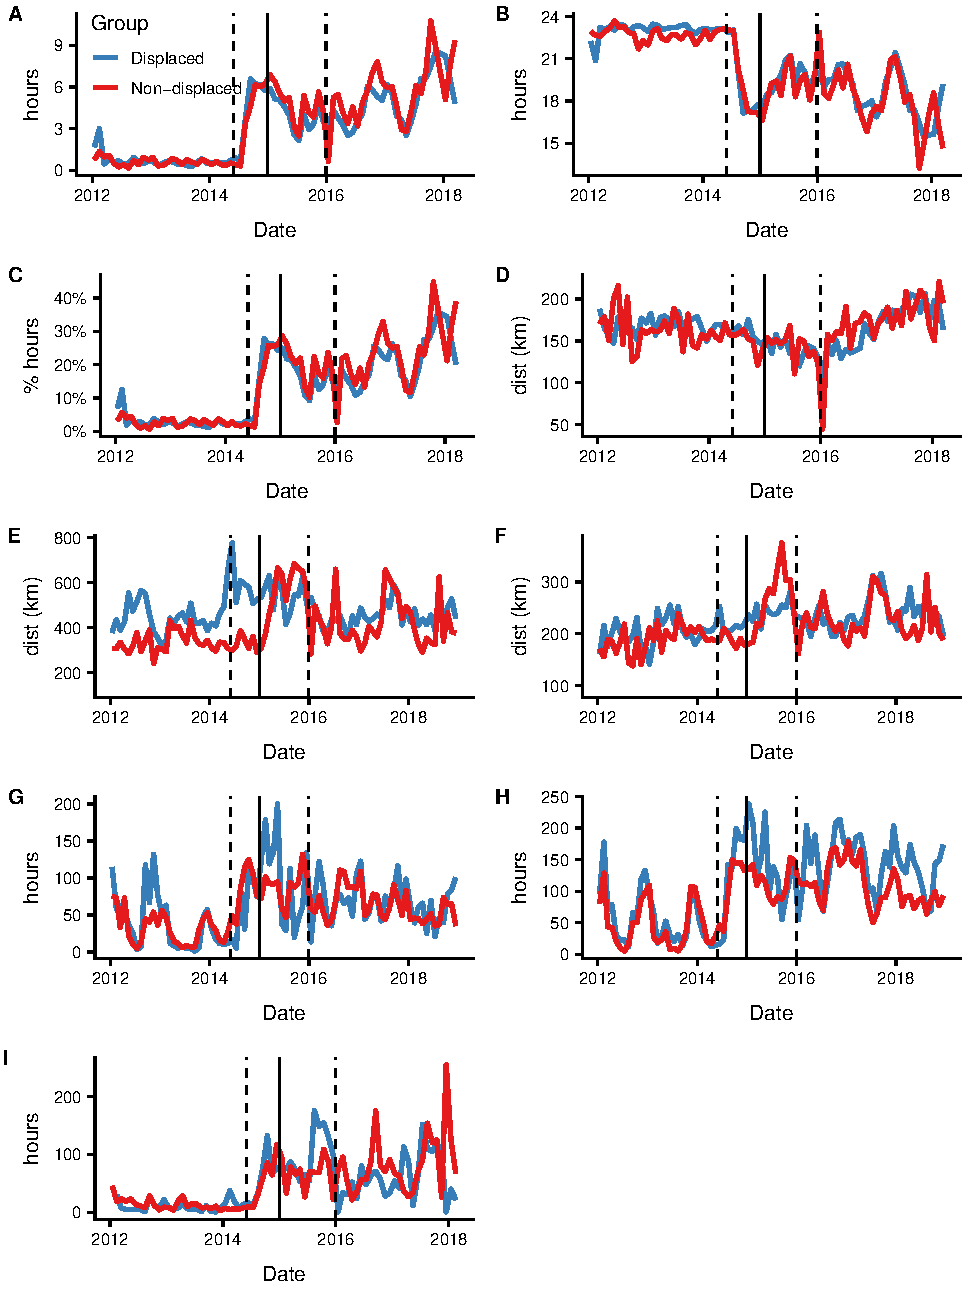
\includegraphics{img/all_panels.pdf}
\caption{\label{fig:all_panels}Time series showing monthly averages for our nine variables of interest: A) Fishing hours, B) Non-fishing hours at-sea, C) Proportion of fishing hours to total hours at-sea, D) Distance traveled, E) Mean distance from port for fishing events, F) Mean distance from shore for fishing events, G) Monthly hours spent in Kiribati waters, H) Monthly hours spent in PNA waters, I) Monthly hours spent on the high seas. Dashed vertical lines indicate the addition of new AIS satellites. Solid vertical line indicates the closure of PIPA.}
\end{figure}

\begin{figure}
\centering
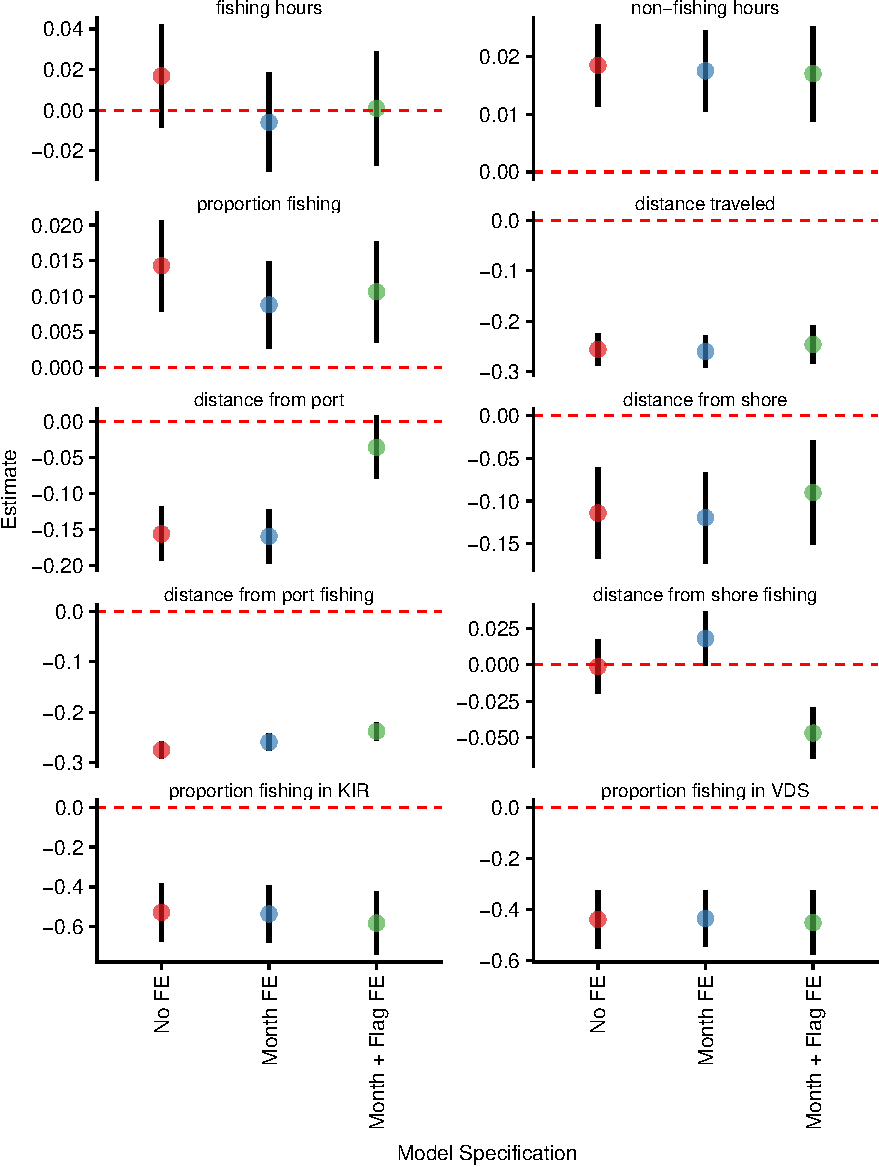
\includegraphics{img/other_specifications.pdf}
\caption{\label{fig:other_specifications}Alternative difference-in-differences estimates for our variables of interest using different model specifications. Table \ref{tab:main_DID} reports estimates for models with month and flag fixed effects, and NINO4 index (\emph{i.e.} green dots).}
\end{figure}

\begin{landscape}

\begin{table}[!htbp] \centering 
  \caption{\label{tab:main_DID}Difference-in-differences estimates for our 10 variables of interest: 1) Daily fishing hours, 2) Daily non-fishing at-sea hours, 3) Daily proportion of fishing hours to total at-sea hours, 4) Daily distance traveled, 5) Daily mean distance from port for fishing events, 6) Daily mean distance from shore for fishing events, 7) Monthly fishing hours spent in Kiribati waters, 8) Monthly fishing hours spent in PNA waters. Numbers in parentheses are heteroskedastic-robust standard errors.} 
  \label{} 
\footnotesize 
\begin{tabular}{@{\extracolsep{1pt}}lcccccccc} 
\\[-1.8ex]\hline 
\hline \\[-1.8ex] 
\\[-1.8ex] & (1) & (2) & (3) & (4) & (5) & (6) & (7) & (8)\\ 
\hline \\[-1.8ex] 
 Constant & 2.449$^{***}$ & 3.325$^{***}$ & 0.314$^{***}$ & 6.177$^{***}$ & 13.800$^{***}$ & 13.159$^{***}$ & 3.979$^{***}$ & 4.644$^{***}$ \\ 
  & (0.061) & (0.031) & (0.014) & (0.042) & (0.047) & (0.065) & (0.392) & (0.343) \\ 
  & & & & & & & & \\ 
 Post & 0.336$^{***}$ & $-$0.353$^{***}$ & 0.083$^{***}$ & 0.105$^{***}$ & 0.398$^{***}$ & 0.352$^{***}$ & 1.151$^{***}$ & 1.240$^{***}$ \\ 
  & (0.024) & (0.015) & (0.006) & (0.020) & (0.016) & (0.016) & (0.157) & (0.125) \\ 
  & & & & & & & & \\ 
 Treated & $-$0.085$^{***}$ & 0.060$^{***}$ & $-$0.028$^{***}$ & 0.259$^{***}$ & 0.259$^{***}$ & 0.163$^{***}$ & 0.435$^{***}$ & 0.082 \\ 
  & (0.027) & (0.014) & (0.007) & (0.020) & (0.018) & (0.018) & (0.163) & (0.133) \\ 
  & & & & & & & & \\ 
 Post $\times$ Treated & 0.036 & $-$0.052$^{***}$ & 0.019$^{***}$ & $-$0.296$^{***}$ & $-$0.342$^{***}$ & $-$0.199$^{***}$ & $-$0.481$^{***}$ & $-$0.335$^{**}$ \\ 
  & (0.028) & (0.017) & (0.007) & (0.024) & (0.020) & (0.019) & (0.179) & (0.142) \\ 
  & & & & & & & & \\ 
\hline \\[-1.8ex] 
Month FE & Yes & Yes & Yes & Yes & Yes & Yes & Yes & Yes \\ 
Flag FE & Yes & Yes & Yes & Yes & Yes & Yes & Yes & Yes \\ 
Observations & 25,004 & 51,724 & 25,004 & 52,767 & 25,004 & 25,004 & 1,399 & 2,010 \\ 
R$^{2}$ & 0.066 & 0.092 & 0.067 & 0.011 & 0.073 & 0.095 & 0.141 & 0.230 \\ 
\hline 
\hline \\[-1.8ex] 
\textit{Note:}  & \multicolumn{8}{r}{$^{*}$p$<$0.1; $^{**}$p$<$0.05; $^{***}$p$<$0.01} \\ 
\end{tabular} 
\end{table} 

\end{landscape}

\begin{landscape}

\begin{table}[!htbp] \centering 
  \caption{\label{tab:main_DID}Difference-in-differences estimates for our 10 variables of interest: 1) Daily fishing hours, 2) Daily non-fishing at-sea hours, 3) Daily proportion of fishing hours to total at-sea hours, 4) Daily distance traveled, 5) Daily mean distance from port for fishing events, 6) Daily mean distance from shore for fishing events, 7) Monthly fishing hours spent in Kiribati waters, 8) Monthly fishing hours spent in PNA waters. Numbers in parentheses are heteroskedastic-robust standard errors.} 
  \label{} 
\footnotesize 
\begin{tabular}{@{\extracolsep{1pt}}lcccccccc} 
\\[-1.8ex]\hline 
\hline \\[-1.8ex] 
\\[-1.8ex] & (1) & (2) & (3) & (4) & (5) & (6) & (7) & (8)\\ 
\hline \\[-1.8ex] 
 Constant & 2.637$^{***}$ & 3.247$^{***}$ & 0.404$^{***}$ & 5.016$^{***}$ & 13.177$^{***}$ & 12.684$^{***}$ & 3.259$^{***}$ & 4.096$^{***}$ \\ 
  & (0.042) & (0.021) & (0.011) & (0.044) & (0.028) & (0.025) & (0.270) & (0.206) \\ 
  & & & & & & & & \\ 
 Post & 0.283$^{***}$ & $-$0.443$^{***}$ & 0.048$^{***}$ & 0.628$^{***}$ & 0.164$^{***}$ & 0.077$^{***}$ & 1.347$^{***}$ & 1.586$^{***}$ \\ 
  & (0.039) & (0.021) & (0.011) & (0.044) & (0.024) & (0.022) & (0.234) & (0.188) \\ 
  & & & & & & & & \\ 
 Treated & $-$0.091$^{**}$ & $-$0.051$^{***}$ & $-$0.052$^{***}$ & 0.683$^{***}$ & 0.137$^{***}$ & $-$0.020 & 0.697$^{***}$ & 0.477$^{***}$ \\ 
  & (0.040) & (0.019) & (0.011) & (0.041) & (0.024) & (0.022) & (0.233) & (0.184) \\ 
  & & & & & & & & \\ 
 Post $\times$ Treated & 0.081$^{*}$ & 0.021 & 0.055$^{***}$ & $-$0.880$^{***}$ & $-$0.153$^{***}$ & 0.017 & $-$0.691$^{***}$ & $-$0.706$^{***}$ \\ 
  & (0.042) & (0.023) & (0.011) & (0.046) & (0.027) & (0.024) & (0.251) & (0.202) \\ 
  & & & & & & & & \\ 
\hline \\[-1.8ex] 
Month FE & Yes & Yes & Yes & Yes & Yes & Yes & Yes & Yes \\ 
Flag FE & Yes & Yes & Yes & Yes & Yes & Yes & Yes & Yes \\ 
Observations & 19,971 & 42,555 & 19,971 & 43,068 & 19,971 & 19,971 & 1,207 & 1,696 \\ 
R$^{2}$ & 0.064 & 0.097 & 0.066 & 0.032 & 0.059 & 0.071 & 0.133 & 0.217 \\ 
\hline 
\hline \\[-1.8ex] 
\textit{Note:}  & \multicolumn{8}{r}{$^{*}$p$<$0.1; $^{**}$p$<$0.05; $^{***}$p$<$0.01} \\ 
\end{tabular} 
\end{table} 

\end{landscape}

\begin{landscape}

\begin{table}[H] \centering 
  \caption{\label{tab:DID_without_USA_TWN}Difference-in-differences estimates for our 9 variables of interest after excluding US and Tawianese vessels. 1) Daily fishing hours, 2) Daily non-fishing at-sea hours, 3) Daily proportion of fishing hours to total at-sea hours, 4) Daily distance traveled, 5) Daily mean distance from port for fishing events, 6) Daily mean distance from shore for fishing events, 7) Monthly fishing hours spent in Kiribati waters, 8) Monthly fishing hours spent in PNA waters, and 9) Monthly fishing hours in the high seas. Numbers in parentheses are heteroskedastic-robust standard errors.} 
  \label{} 
\footnotesize 
\begin{tabular}{@{\extracolsep{1pt}}lccccccccc} 
\\[-1.8ex]\hline 
\hline \\[-1.8ex] 
\\[-1.8ex] & (1) & (2) & (3) & (4) & (5) & (6) & (7) & (8) & (9)\\ 
\hline \\[-1.8ex] 
 Constant & 0.536$^{***}$ & 3.600$^{***}$ & 0.082$^{***}$ & 4.506$^{***}$ & 13.002$^{***}$ & 12.438$^{***}$ & 3.850$^{***}$ & 4.719$^{***}$ & 2.420$^{***}$ \\ 
  & (0.023) & (0.012) & (0.004) & (0.043) & (0.022) & (0.020) & (0.209) & (0.158) & (0.419) \\ 
  & & & & & & & & & \\ 
 Post & 0.796$^{***}$ & $-$0.217$^{***}$ & 0.130$^{***}$ & 0.021 & 0.290$^{***}$ & 0.291$^{***}$ & 0.870$^{***}$ & 0.894$^{***}$ & 0.732$^{**}$ \\ 
  & (0.019) & (0.010) & (0.003) & (0.035) & (0.016) & (0.016) & (0.156) & (0.121) & (0.291) \\ 
  & & & & & & & & & \\ 
 Displaced & 0.142$^{***}$ & 0.016$^{**}$ & 0.015$^{***}$ & 0.341$^{***}$ & 0.227$^{***}$ & 0.127$^{***}$ & 0.490$^{***}$ & $-$0.017 & $-$0.296 \\ 
  & (0.013) & (0.007) & (0.002) & (0.031) & (0.018) & (0.017) & (0.163) & (0.126) & (0.239) \\ 
  & & & & & & & & & \\ 
 NINO4 & $-$0.001 & $-$0.001 & 0.001 & $-$0.383$^{***}$ & 0.189$^{***}$ & 0.082$^{***}$ & 0.325$^{***}$ & 0.171$^{***}$ & 0.441$^{***}$ \\ 
  & (0.011) & (0.006) & (0.002) & (0.019) & (0.009) & (0.008) & (0.075) & (0.063) & (0.122) \\ 
  & & & & & & & & & \\ 
 Post $\times$ Displaced & $-$0.212$^{***}$ & $-$0.002 & $-$0.029$^{***}$ & $-$0.158$^{***}$ & $-$0.328$^{***}$ & $-$0.184$^{***}$ & $-$0.533$^{***}$ & $-$0.225 & 0.339 \\ 
  & (0.021) & (0.010) & (0.004) & (0.039) & (0.019) & (0.018) & (0.175) & (0.138) & (0.291) \\ 
  & & & & & & & & & \\ 
\hline \\[-1.8ex] 
Month FE & Yes & Yes & Yes & Yes & Yes & Yes & Yes & Yes & Yes \\ 
Flag FE & Yes & Yes & Yes & Yes & Yes & Yes & Yes & Yes & Yes \\ 
Observations & 73,717 & 73,717 & 73,716 & 73,778 & 26,920 & 26,920 & 1,546 & 2,236 & 660 \\ 
R$^{2}$ & 0.095 & 0.072 & 0.102 & 0.021 & 0.077 & 0.094 & 0.111 & 0.169 & 0.256 \\ 
\hline 
\hline \\[-1.8ex] 
\textit{Note:}  & \multicolumn{9}{r}{$^{*}$p$<$0.1; $^{**}$p$<$0.05; $^{***}$p$<$0.01} \\ 
\end{tabular} 
\end{table} 

\end{landscape}

\begin{figure}
\centering
	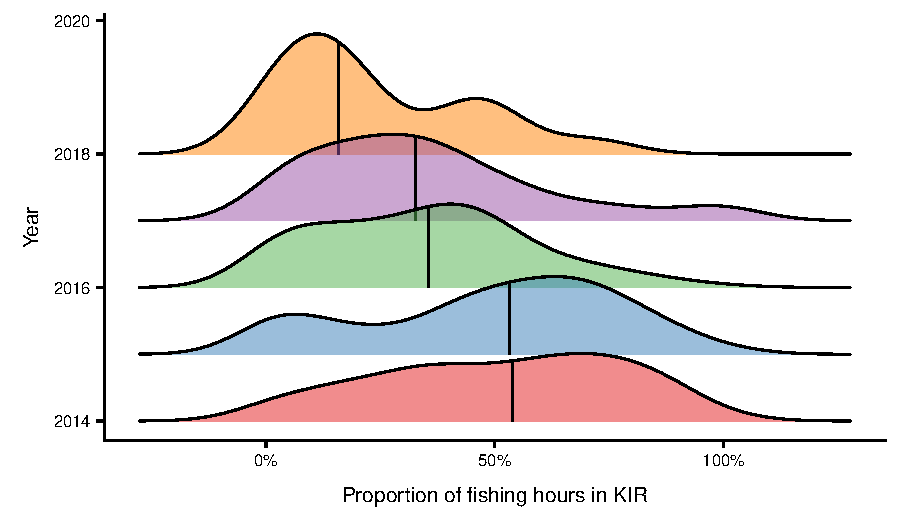
\includegraphics{img/hist_kir_fishing.pdf}
	\caption{\label{fig:hist_kir_fishing}Ridgeplot for the density of the \% of total fishing hours that take place within Kiribati EEZ waters by year for displaced vessels where the unit of observation is an individual vessel.}	
\end{figure}

\begin{figure}
\centering
	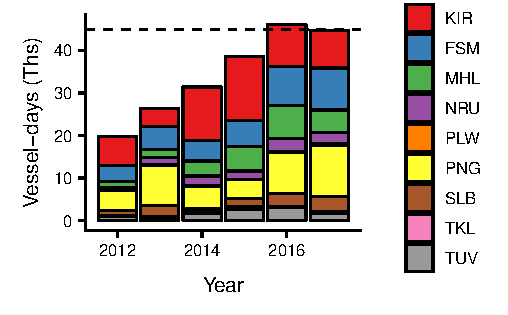
\includegraphics{img/all_PS_VDS_cty_year.pdf}
	\caption{\label{fig:all_PS_VDS_cty_year}Annual vessel-days for all PNA countries, by country.}
\end{figure}

\begin{figure}
\centering
	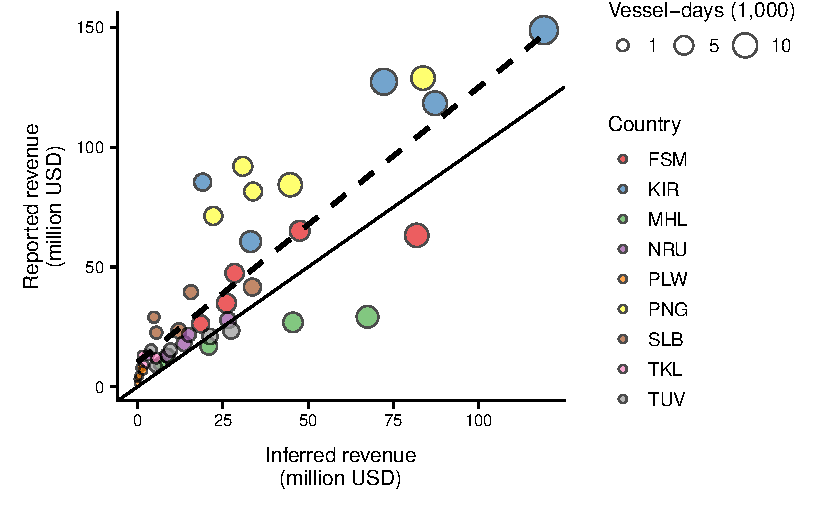
\includegraphics{img/revenue_FFA_GFW_linear.pdf}
	\caption{\label{fig:revenue_FFA_GFW_linear}Inferred revenues vs. reported revenues. The dashed line represents line of best fit, and the solid line represents a 1:1 line.}
\end{figure}

\begin{figure}
\centering
	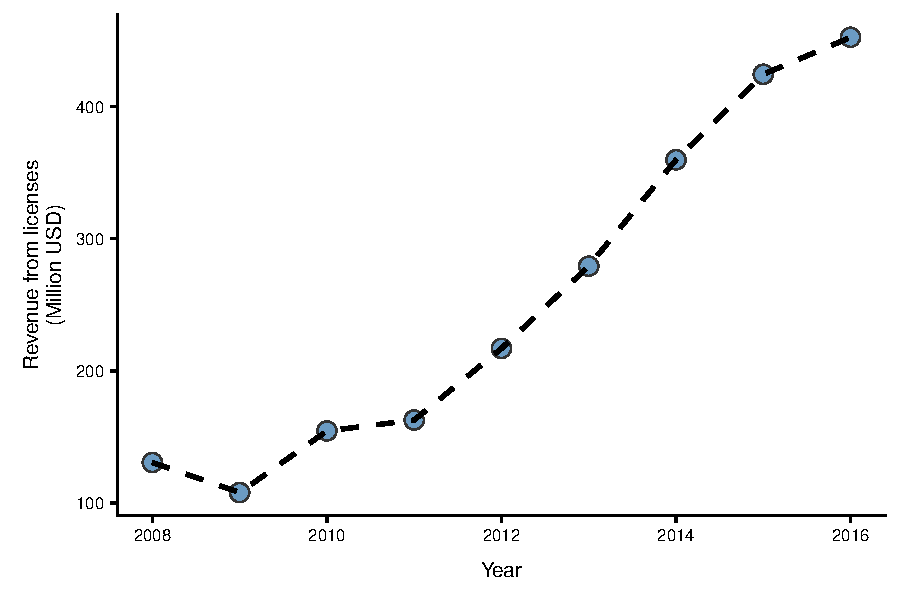
\includegraphics{img/total_PNA_revenues.pdf}
	\caption{\label{fig:total_PNA_revenues}Total revenues for all PNA countries combined.}
\end{figure}

\begin{figure}
\centering
	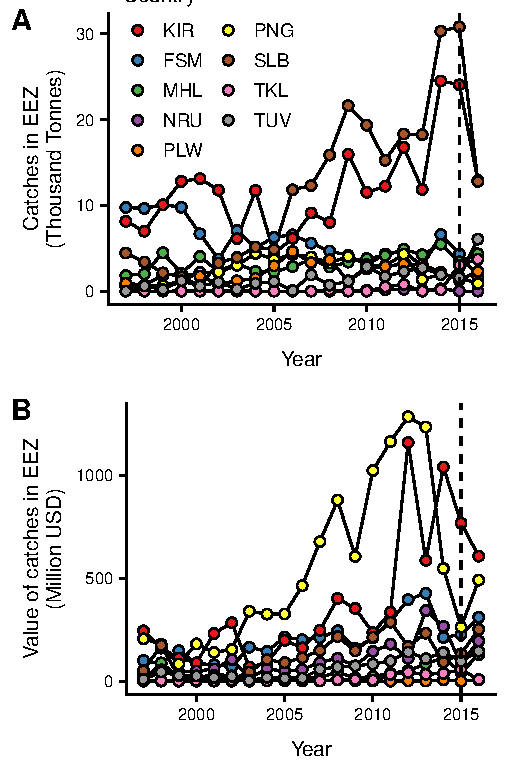
\includegraphics{img/catches.pdf}
	\caption{\label{fig:catches}Financial indicators for PNA countries. A) Total annual purse seine catch by EEZ and, B) Total annual value of purse seine catch by EEZ. Vertical dashed line in both plots denotes implementation of PIPA.}
\end{figure}

\begin{figure}
\centering
	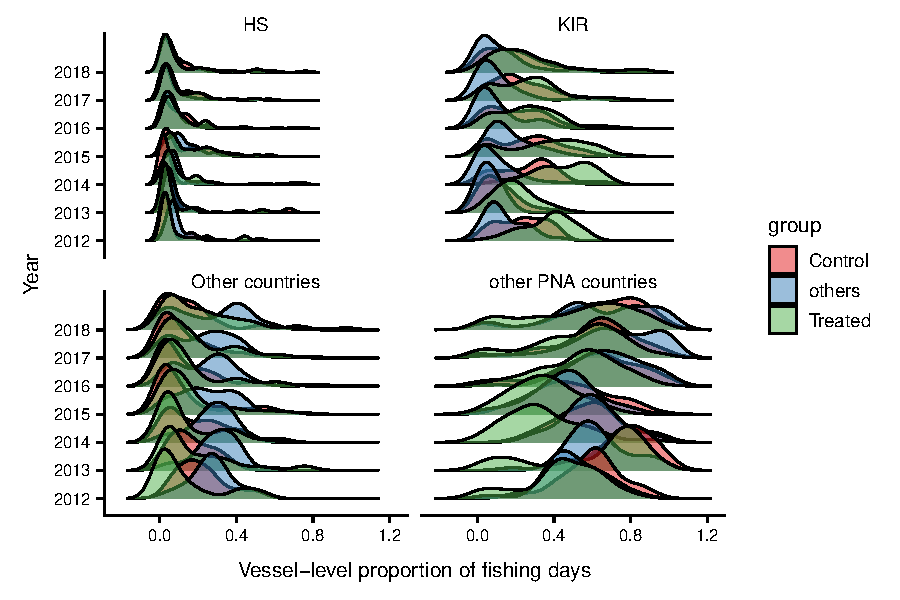
\includegraphics{img/yearly_distribution_prop_fishing_by_region.pdf}
	\caption{\label{fig:yearly_distribution_prop_fishing_by_region}Ridgeplot for the density of the \% of total fishing hours that take place in each region for all vessels}	
\end{figure}

\clearpage

\begin{figure}
\centering
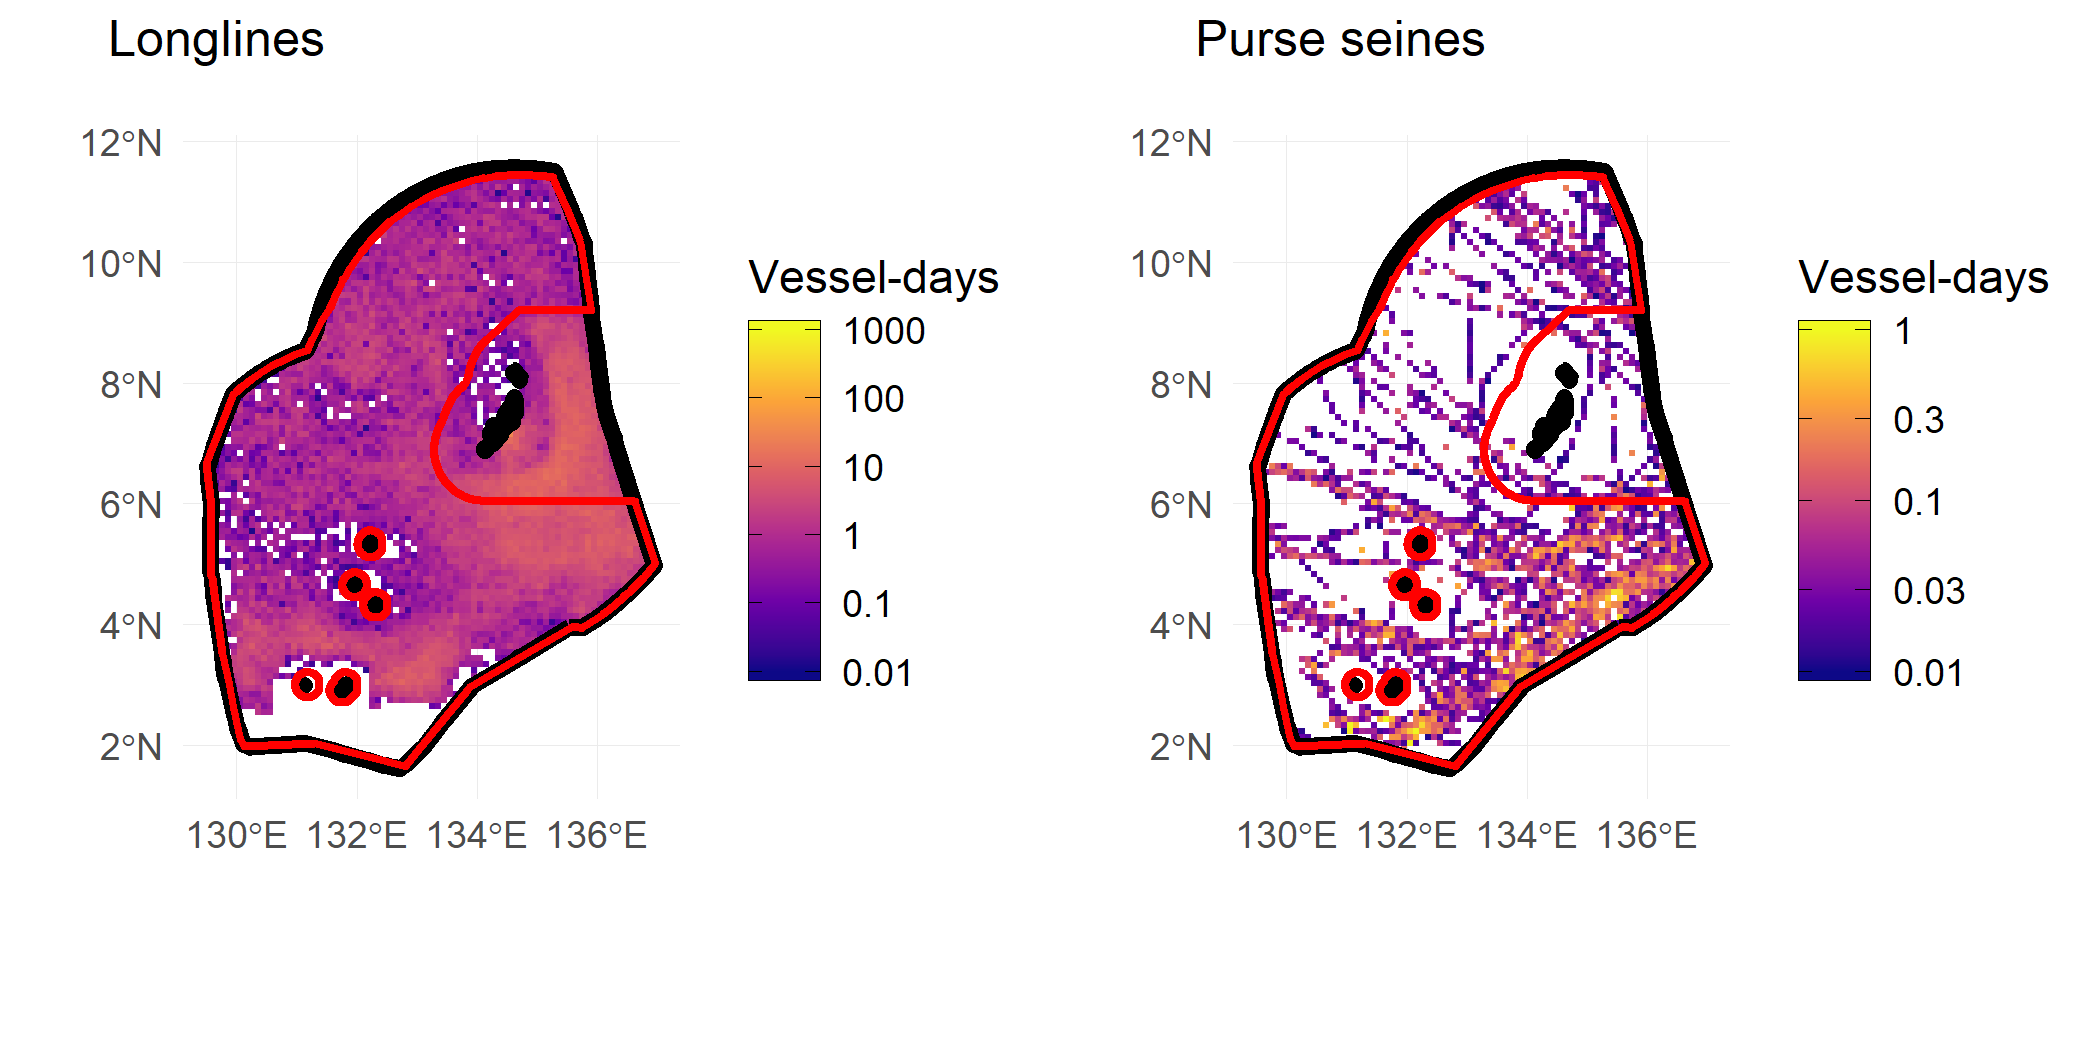
\includegraphics{img/plw_2018.png}
\caption{\label{fig:plw_2018}Longline and purse seine fishing effort in Palaw during 2018 at a 0.5 degree resolution. The red polygon shows the Palau National Marine Sanctuary.}
\end{figure}

I used this figure at the workshop last week, I do not intend to use it with the current design. I want to have a normal white background and split it into 2 (longliners and purse seiners) to better capture the effort that would be displaced by PNMS. I might also break it by year (2015 - 2018) to show that patterns are consistent through time.


\begin{figure}
\centering
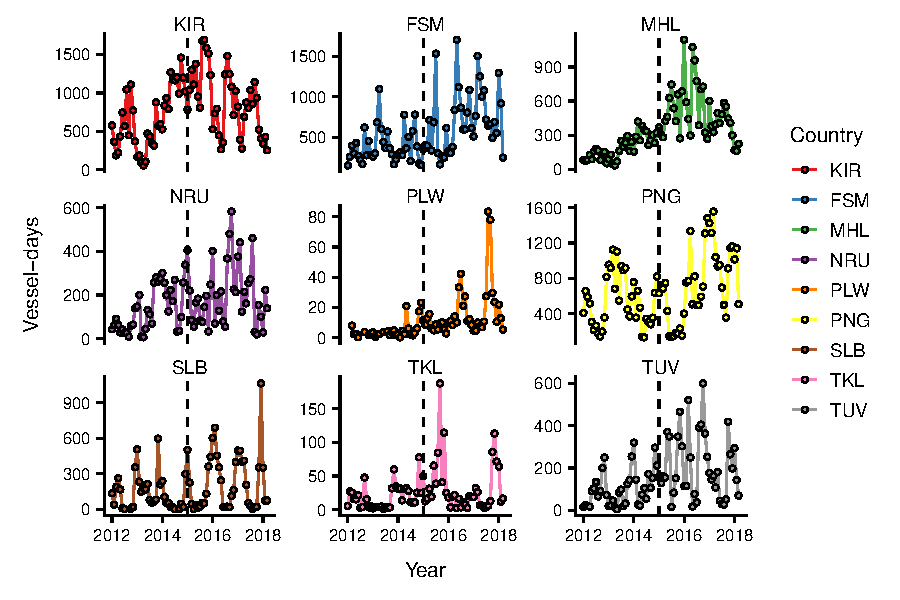
\includegraphics{img/PS_VDS_PNA_by_month_eez.pdf}
\caption{\label{PS_VDS_PNA_by_month_eez}Time series of monthly observed vessel-days for each PNA country.}
\end{figure}

\begin{figure}
\centering
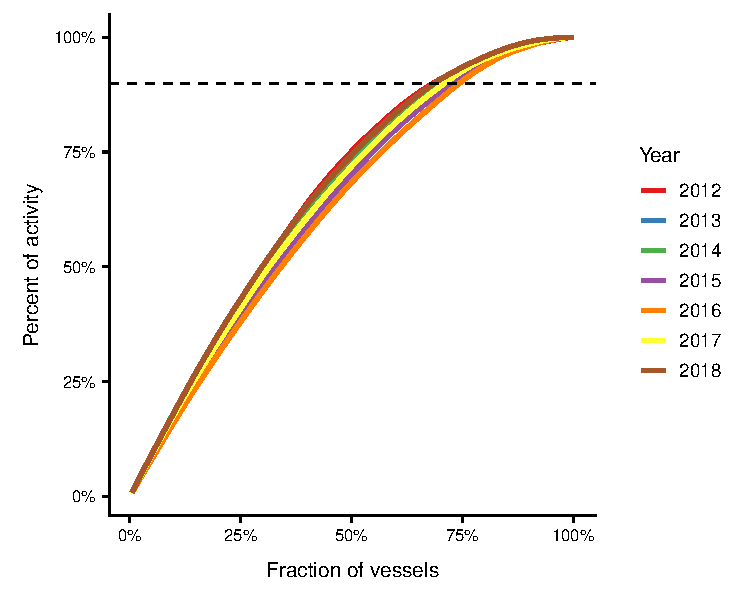
\includegraphics{img/nvessels_to_90.pdf}
\caption{\label{fig:nvessels_to_90}Cumulative activity (\% of total hours) as a function of increasing fraction of vessels (\% of total) by year.)}
\end{figure}



%\section{Old Text}

%\subsection{Large-Scale Marine Protected Areas}\label{lsmpas}
%
%The cutoff at which an MPA is considered to be a LSMPA ranges from areas
%larger than 30,000 km\textsuperscript{2} as defined by
%\cite{desanto_2013} or areas larger than 250,000 km\textsuperscript{2},
%as defined by \cite{toonen_2013}. Figure \ref{fig:LSMPAs_map} shows
%LSMPAs that meet the latter condition, and are also fully no-take. LSMPAs are often
%implemented in the pelagic environment, where the dominant human
%activity is industrial fishing \cite{gray_2017,kroodsma_2018}. The
%early literature on LSMPAs focused on the inherent challenges and
%difficulties that come with a pelagic environment. \cite{kaplan_2010}
%claimed that very large MPAs would result in excessive opportunity costs
%and that these would be difficult to enforce. \cite{game_2009}
%suggested that most of the challenges could be overcome with the
%incorporation of technology, in what then became known as Dynamic Ocean
%Management \cite{maxwell_2015}.\footnote{See \cite{singleton_2014}, who provide an objective discussion of the pros and cons of LSMPAs.} 
%
%Spatial closures of this magnitude are likely to induce changes in
%fishers' behavior. Theoretical models of fishing effort redistribution
%range from the simplistic assumption that effort inside the bounded
%region disappears, to spatially explicit models that reallocate fishing
%effort based on habitat characteristics, presence of other vessels, and
%expected returns \cite{smith_2003,hilborn_2006}. However, these focus
%on the long term optimal equilibrium, and redistribution of fishing
%effort may not always be optimally distributed, especially over the first few years
%\cite{stevenson_2013}.
%
%The empirical research that has been done in smaller sized MPAs
%suggests that resource users may show idiosyncratic responses. For
%example, \cite{stevenson_2013} show that a network of MPAs displaced
%fishing effort farther away from ports, resulting in higher
%\emph{perceived} costs, and increases in catch per unit effort.
%\cite{cabral_2017} analyze the redistribution of fishing and
%non-fishing vessels following the implementation of a network of MPAs in
%California, and find that dive boats follow a
%fishing-the-line pattern, while some fishing boats follow an ideal free
%distribution. More recently \cite{elahi_2018} used satellite tracking
%data to show that a temporal spatial closure caused trawlers to maintain
%effort but apply it more intensively elsewhere, particularly along the
%borders and closer to shore. The way in which fishers react to a spatial
%closure can have major implications for its outcome
%\cite{smith_2003,hilborn_2006}, highlighting the need to understand how
%fishers react to the implementation of LSMPAs, how fishing effort
%changes, and how it is spatially redistributed. All these studies evaluate relatively small closures within Exclusive Economic Zones, where other regulations exist.
%This may not always be the case for LSMPAs, where often the entire EEZ
%is converted into a LSMPA, leaving fishers with the option of moving to
%the high seas or other countries' EEZs, with potentially very different fishing regulations.
%
%\subsection{Nauru agreement and the Phoenix Islands Protected Area}
%
%The cooperation that emerged under the Nauru Agreement allowed for subsequent
%agreements that strengthened fisheries management, like the Palau
%Agreement, which limited the number of purse seiners at 205 vessels from
%1995-2007.\footnote{See \cite{havice_2010} for a detailed description of the Nauru, Palau, and Federated States of Micronesia agreements.} However, the most notable regulation is
%the approach to manage fishing effort: a Vessel Day Scheme (VDS)
%implemented in 2007 \cite{havice_2013}. This effectively modified how
%fishing effort was managed, from total number of vessels (under the Palau
%Agreement) to total vessel-days. 
%Under the purse seine VDS, a total number of annual vessel days for the entire fishery is agreed upon by the PNA parties. Each party’s allowable effort (PAE) is then calculated based on historic effort and biomass within each party’s EEZ. Sixty percent of the PAE is calculated based on EEZ effort over the last seven years and 40\% of the PAE is calculated based on the 10-year average of each country’s share of estimated skipjack and yellowfin biomass within its EEZ.\footnote{This is explained in more detail in Article 12.5 of the 2012 Amendment to the Palau Agreement and in \cite{Hagrannsoknir2014}}. A minimum benchmark fee is set for purse seine vessel days which each party can transfer (\emph{i.e.} sell to another PNA member) or sell to the highest bidder (\emph{i.e.} sell to a fishing company). Vessel days can be transferred to fish in any PNA party’s EEZ, without penalty to the transferred parties' allocations \cite{PNA2016}.\footnote{The process of transferring days between parties is described in Article 7 of the Management Scheme \cite{PNA2016}.} The mean value of a vessel day has steadily increased since 2007 \cite{havice_2013}. 
%Although detailed records on sales or transfers of vessel days are not publicly available \cite{havice_2013,yeeting2018stabilising}, a minimum benchmark fee of \$8,000/day was set from 2015 \cite{PNA2014a}.
%
%\cite{yeeting2018stabilising} summarize the PNA implementing arrangements as follows: “foreign vessels [are required] to be registered and licensed, report catches, maintain log books, allow observers on board and maintain transparency over their fishing activities.” Further, vessels registered with the Vessel Day Scheme are required to have Automatic Location Communicators (ALC) or Mobile Transceiver Units (MTU) that transmit their locations at least once per hour while they are within the VDS Management Area \cite{PNA2016}. Every entire day that a vessel is within the VDS Management Area is counted as a vessel day used, unless the vessel reports a “no fishing day” (e.g., travel, maintenance, etc.) and periods of less than 24 hours are counted as partial days \cite{PNA2016}.  As described in the Palau Arrangement, fishing days by vessels shorter than 50m (longer than 80m) count as 0.5 (1.5) vessel days. Countries are responsible for ensuring registered vessels comply with the implementing arrangements and that they stay within their PAE. Parties that exceed their PAE should reportedly be penalized by reductions to the following year’s PAE \cite{PNA2016}. There are some criticisms of the PNA PS VDS claiming that there is a lack of monitoring, compliance, and transparency that could hinder the future success of the program \cite{Arnason2014,yeeting2018stabilising}. While the effectiveness of this scheme has been
%debated in terms of meeting fishery management and conservation
%objectives, the licensing significantly contributes to the economy of
%these island nations \cite{havice_2010}.
%
%The main tuna species caught in the region are skipjack
%(\emph{Katsuwonus pelamis}), yellowfin (\emph{Thunnus albacares}),
%albacore (\emph{Thunnus alalunga}) and bigeye (\emph{Thunnus obesus}).
%From these, the first two are amongst the top-10 species represented in
%global fisheries production statistics, with 2016 catches increasing
%relative to the 2005-2014 average \cite{fao_2018}. This region of the
%Pacific has historically accounted for a large portion of tuna catches
%\cite{aqorau_1997}. Today, the PNA controls close to 50\% of global
%skipjack tuna production \cite{pna_website_2018} and the combined area of all EEZs involved is 14.6 million km\textsuperscript{2}, larger than the land mass of the United States of America. A large portion of global skipjack
%catch derives from purse seine vessels licensed under the VDS.
%Fishing vessels from Australia, New Zealand, China, France, Korea,
%Japan, the Philippines, Taiwan, and the United States participate in the
%purse-seining VDS.
%
%One of the most notable and recent management interventions in the
%region is the implementation of the Phoenix Islands Protected Area (PIPA)
%by the government of Kiribati. PIPA was first declared in 2006, and
%established in 2008 with only 4\% of the area declared as no-take. On
%January 1\textsuperscript{st}, 2015, the no-take area within PIPA was
%expanded to a total area of 397,447 km\textsuperscript{2}, roughly 1.5
%times the size of Ecuador. Figure \ref{fig:PNA_map} shows a map of the
%PNA countries (excluding Palau) and the Phoenix Islands Protected Area.
%
%The closure of such a large area in one of the most important fishing
%regions in the world provides a unique opportunity to evaluate the
%behavioral responses and redistribution of fishing effort by vessels
%that used to fish there. PIPA has been the focus of previous research
%showing that fishing effort is effectively reduced after implementation
%\cite{mccauley_2016,mcdermott_2018}. To this, we pose two questions:
%How did individual vessels respond to the sudden exclusion of such a big
%area? Where did all the vessels go? And what does this imply for revenues from
%selling VDS for both Kiribati and the PNA as a whole? 
%
%A spatial closure might cause fishers to modify
%their behavior as they adapt to a new state of the world. For example, some may have
%to travel further distances to find new fishing grounds, increasing their fuel
%costs. If fishers had developed experience for fishing in particular
%sites, being excluded might impose a learning cost on them, as they
%identify new fishing grounds. This might result in increased search
%times. However, if the area of knowledge of a vessel is significantly
%larger than that of the spatial closure, they might already know other
%places to fish. In the next sections we describe
%the data and methods used to answer these questions.
%
%\subsection{Palau}
%
%\subsubsection{Palau National Monument}

%On October 28, 2015, the President of Palau, H.E. Tommy E. Remengesau Jr., signed into law the Palau National Marine Sanctuary (PNMS) Act. Starting in December 2020, this Act will close 500,000 km\textsuperscript{2} to commercial fishing activities, creating the 14th largest protected area in the world. The sanctuary will fully protect about 80 percent of the nation’s EEZ. The remaining 20\% of Palau’s EEZ (close to the most heavily populated islands: Koror and Babeldaob) will become a Domestic Fishing Zone in which traditional and domestic fishing activities will be allowed to provide fish solely for the domestic market (\emph{i.e.} exports of pelagic fish will be prohibited). Alongside these protections, the Palau National Marine Sanctuary (PNMS) Act will support a domestic pelagic fishery. In this section, we use our preceding analysis on the ex-post impacts of PIPA to attempt to make some \emph{ex ante} predictions about the potential impacts of PNMS. We start by giving some background on the fishing that is currently taking place inside the future PNMS. 

%\subsubsection{Background on Commercial Fishing in Palau}

%Foreign tuna fishing in Palau’s EEZ began before WWI. Pole and line was the initial gear used to target skipjack tuna by Japanese vessels. Foreign fishing activities stopped during WWII and started again in the 1960s when Japanese fishers returned and the locally based Van Camp Seafood Company carried out fishing with boats crewed by Okinawans. The Japanese also began purse seine fishing in the 1960s and 1970s and limited longline fishing for yellowfin tuna developed during the same time. During the 1980s, longline fishers began to set their lines deeper, shifting their targets to bigeye tuna. During the 1980s, Korean and Taiwanese vessels also began longline fishing in Palauan waters for export to Japan \cite{chapman2000development}. There are currently three transshipment companies operating in Palau.

%Purse seine vessels target schools of skipjack tuna that are then canned. Compared to other EEZs in the Pacific, especially the PNA EEZs, Palau’s EEZ is not known to be a preferred fishing ground for purse seining (Sisior, pers. comm.). This can be seen in Figure \ref{fig:VDS_country_year}. Currently all purse seine boats fishing in Palau’s EEZ are Japanese and they do not land their catch in Palau (Table \ref{tab:palau_purse}). 



%All longline vessels fishing in Palau’s EEZ are foreign owned (Table \ref{tab:palau_long}). Japanese longline vessels do not land their catch in Palau. Locally-based, foreign-owned longline boats are mostly Taiwanese vessels that are contracted by one of the two main fishing companies (Palau International Traders Incorporated (PITI) and Kuniyoshi Fishing Company (KFC)). Ninety-five percent of the catch from PITI and KFC contracted boats is exported to Japan upon landing in Koror (the largest town in and former capital of Palau). Most of the discards are either sold or donated in Palau. A very small portion of the discards is frozen and transported to Taiwan when vessels return to their home ports.



%\subsubsection{Access fees and taxes}
%
%An agreement between Palau and four Japanese fishing associations\footnote{This is a single agreement between Palau and four associations—1)Federation of Japan Tuna Fisheries Cooperative Associations, 2) National Offshore Tuna Fisheries Association of Japan, 3) Japan Far Seas Purse Seine Fishing Association, 4) Federation of North Pacific District Purse Seine Fisheries Cooperative Association of Japan (Performance Audit Report on Managing Sustainable Fisheries (Tuna) 2013).} covered three methods of fishing (longline, purse seine, and pole and line) and allowed Japan to have up to 290 vessels in Palau waters with no limits on catch. Japan paid 4-5\% of catch returns for this access, but there was no way to validate their catch \cite{Tewid2013}. Between 2010 and 2014, Japan paid Palau between \$196,100- \$867,120 annually in access fees \cite{Gillett2016}. Currently, these access fees have been replaced by the PNA vessel day scheme (described earlier).
% 
%There used to be a number of agreements between the Republic of Palau and foreign owned, local based companies, in particular PITI and KFC, to allow longline fishing \cite{Tewid2013}. Vessels under these agreements were internationally-owned, locally-based vessels that paid for annual licenses based on the size of each vessel. These are the vessels shown in Table \ref{tab:palau_long} (excluding the Japanese vessels). So, for example, there were 38 vessels as part of these agreements in 2016. Between 2010 and 2014, licensing fee revenue from these agreements was between \$219,000-\$284,600 per year \cite{Gillett2016}. These access fees have also been replaced by a new longline-specific version of the VDS (described in more detail below).
%
%There are two multilateral treaties that grant preferential access to Palau waters to US and Federated States of Micronesia (FSM) flagged purse seine boats: the US Multilateral Tuna Treaty and the Federated States of Micronesia Arrangement.  The US Treaty was renegotiated in 2016 with stipulations on minimum vessel day fees. Very little purse seine fishing is conducted by FSM and US vessels in Palau’s EEZ, but Palau still receives a portion of these treaty funds. These agreements have been described by some commentators as foreign aid, with little connection to underlying fish stocks \cite{Gillett2016}. 
%
%The export tax for all commercial tuna and billfish, either fresh or frozen, is \$0.35/kg. Average annual revenue from export taxes was around \$500,000 from 2011-2014 \cite{Gillett2016}. 
%Other than the access fees and tax revenue, Palau receives little additional economic benefits from pelagic fisheries, especially considering that very few jobs are created by the fishery. Between 80 to 90 people are employed by offshore fisheries, and of these only around 20\% are Palauans, earning wages that are only 50\% of average wages in Palau \cite{Gillett2016}.
%
%\subsubsection{Parties to the Nauru Agreement and the Vessel Day Scheme}
%
%In the case of Palau, the VDS is run by the Bureau of Marine Resources, within the Ministry of Natural Resources, Environment and Tourism. Palau’s current purse seine VDS allotment is reportedly around 700 vessel days annually (Sisior, pers. comm., \cite{Pojas2018}), although historically this number has been lower (average of 580 days between 2008-2011 \cite{Tewid2013}). Palau sells most of its vessel days to the US for \$12,500 per day (as negotiated in the US treaty), regardless of whether US vessels actually fish in Palau’s EEZ. The remainder of Palau’s purse seine vessel days are sold for between \$9-10,000 each. When vessel days are purchased to transfer to another EEZ, Palau charges a transfer fee (approximately \$500), for administration costs and future opportunity costs (since vessel day allotments are based partly on historical effort within the EEZ). Though records are confidential, it has been publicly reported that one PNA member party that Palau has transferred vessel days to is Papua New Guinea \cite{Tewid2013} and in 2018, vessel days were sold to a fishing company in the Philippines for the first time \cite{Pojas2018}. In 2018, Palau brought in approximately \$9 million USD in VDS revenue (Sisior pers. comm.). 
%
%The longline VDS (LL VDS) is in its infancy and has not yet been fully implemented at the PNA-scale, although several countries are now implementing it at the country-scale. Palau was the first party to implement the VDS for longline fishing in 2017. In 2014, longline boats fishing in Palau’s EEZ fished 10,500 days (Sisior, pers. comm.). Since 2016, the number of allowed longline VDs has been a fraction of the 2014 days, reducing each year as stipulated in the PNMS Act. Palau sells its LL VD for \$150-\$250 (Sisior pers. comm.). Because the LL VDS is still new and has yet to be fully implemented by all parties, LL VD are not currently transferable between PNA member EEZs. 
%
%\subsubsection{Plans for a domestic pelagic fishery}
%
%In the recent past, a single domestic pole and line vessel supplied Palau with an estimated 100mt of catch \cite{Gillett2016}. The vessel ceased operations in recent years when the captain became ill and passed away, but there is talk that it is gearing up to start operations again under new leadership (Sisior, pers. comm.). Otherwise, there are no domestic vessels dedicated to full-time offshore fishing. A number of fishers occasionally troll offshore for tuna and other pelagics, but there are no official estimates of volumes. 
%Local NGOs have sponsored short trainings on small-scale canning and proper techniques for processing high grade tuna to encourage existing fishers to devote more time to offshore fishing. There are several possible scenarios for a domestic fishery (including those featured in a feasibility report by FFA \cite{Skirtun2017}), but there has yet to be any official action towards a particular scenario.

\end{document}
